% Options for packages loaded elsewhere
\PassOptionsToPackage{unicode}{hyperref}
\PassOptionsToPackage{hyphens}{url}
%
\documentclass[
]{ltjsarticle}
\usepackage{lmodern}
\usepackage{amssymb,amsmath}
\usepackage{ifxetex,ifluatex,ifpdf,ifthen}
\ifnum 0\ifxetex 1\fi\ifluatex 1\fi=0 % if pdftex
  \usepackage[T1]{fontenc}
  \usepackage[utf8]{inputenc}
  \usepackage{textcomp} % provide euro and other symbols
\else % if luatex or xetex
  \usepackage{unicode-math}
  \defaultfontfeatures{Scale=MatchLowercase}
  \defaultfontfeatures[\rmfamily]{Ligatures=TeX,Scale=1}
\fi

% japanese font setting
% if the preset is specified
\ifxetex
  \usepackage[AutoFallBack=true]{zxjatype}
  \usepackage[noto,]{zxjafont}
  \usepackage{xeCJKfntef}
\fi
\ifluatex
  \usepackage{luatexja}
  \usepackage[,noto]{luatexja-preset}
  %\renewcommand{\kanjifamilydefault}{\gtdefault}
\fi

  \IfFileExists{pxrubrica.sty}{\usepackage{pxrubrica}}{}
\ifluatex
  \ltjsetparameter{%
    jacharrange={-2,-3},
    alxspmode={`/,allow},
    alxspmode={`#,allow},
    alxspmode={92,allow}
  }
\fi


% Use upquote if available, for straight quotes in verbatim environments
\IfFileExists{upquote.sty}{\usepackage{upquote}}{}
\ifpdf
  \IfFileExists{microtype.sty}{% use microtype if available
    \usepackage[]{microtype}
    \UseMicrotypeSet[protrusion]{basicmath} % disable protrusion for tt fonts
  }{}
\fi
\makeatletter
\@ifundefined{KOMAClassName}{% if non-KOMA class
  \IfFileExists{parskip.sty}{%
    \usepackage{parskip}
  }{% else
    \setlength{\parindent}{0pt}
    \setlength{\parskip}{6pt plus 2pt minus 1pt}}
}{% if KOMA class
  \KOMAoptions{parskip=half}}
\makeatother
\usepackage{xcolor}
\IfFileExists{xurl.sty}{\usepackage{xurl}}{} % add URL line breaks if available
\IfFileExists{bookmark.sty}{\usepackage{bookmark}}{\usepackage{hyperref}}
\hypersetup{
  pdftitle={R Markdown 入門 (Tokyo.R \#91)},
  pdfauthor={ill-identified},
  hidelinks,
  pdfcreator={LaTeX via pandoc}}
\urlstyle{same} % disable monospaced font for URLs
\usepackage{color}
\usepackage{fancyvrb}
\newcommand{\VerbBar}{|}
\newcommand{\VERB}{\Verb[commandchars=\\\{\}]}
\DefineVerbatimEnvironment{Highlighting}{Verbatim}{commandchars=\\\{\}}
% Add ',fontsize=\small' for more characters per line
\usepackage{framed}
\definecolor{shadecolor}{RGB}{248,248,248}
\newenvironment{Shaded}{\begin{snugshade}}{\end{snugshade}}
\newcommand{\AlertTok}[1]{\textcolor[rgb]{0.94,0.16,0.16}{#1}}
\newcommand{\AnnotationTok}[1]{\textcolor[rgb]{0.56,0.35,0.01}{\textbf{\textit{#1}}}}
\newcommand{\AttributeTok}[1]{\textcolor[rgb]{0.77,0.63,0.00}{#1}}
\newcommand{\BaseNTok}[1]{\textcolor[rgb]{0.00,0.00,0.81}{#1}}
\newcommand{\BuiltInTok}[1]{#1}
\newcommand{\CharTok}[1]{\textcolor[rgb]{0.31,0.60,0.02}{#1}}
\newcommand{\CommentTok}[1]{\textcolor[rgb]{0.56,0.35,0.01}{\textit{#1}}}
\newcommand{\CommentVarTok}[1]{\textcolor[rgb]{0.56,0.35,0.01}{\textbf{\textit{#1}}}}
\newcommand{\ConstantTok}[1]{\textcolor[rgb]{0.00,0.00,0.00}{#1}}
\newcommand{\ControlFlowTok}[1]{\textcolor[rgb]{0.13,0.29,0.53}{\textbf{#1}}}
\newcommand{\DataTypeTok}[1]{\textcolor[rgb]{0.13,0.29,0.53}{#1}}
\newcommand{\DecValTok}[1]{\textcolor[rgb]{0.00,0.00,0.81}{#1}}
\newcommand{\DocumentationTok}[1]{\textcolor[rgb]{0.56,0.35,0.01}{\textbf{\textit{#1}}}}
\newcommand{\ErrorTok}[1]{\textcolor[rgb]{0.64,0.00,0.00}{\textbf{#1}}}
\newcommand{\ExtensionTok}[1]{#1}
\newcommand{\FloatTok}[1]{\textcolor[rgb]{0.00,0.00,0.81}{#1}}
\newcommand{\FunctionTok}[1]{\textcolor[rgb]{0.00,0.00,0.00}{#1}}
\newcommand{\ImportTok}[1]{#1}
\newcommand{\InformationTok}[1]{\textcolor[rgb]{0.56,0.35,0.01}{\textbf{\textit{#1}}}}
\newcommand{\KeywordTok}[1]{\textcolor[rgb]{0.13,0.29,0.53}{\textbf{#1}}}
\newcommand{\NormalTok}[1]{#1}
\newcommand{\OperatorTok}[1]{\textcolor[rgb]{0.81,0.36,0.00}{\textbf{#1}}}
\newcommand{\OtherTok}[1]{\textcolor[rgb]{0.56,0.35,0.01}{#1}}
\newcommand{\PreprocessorTok}[1]{\textcolor[rgb]{0.56,0.35,0.01}{\textit{#1}}}
\newcommand{\RegionMarkerTok}[1]{#1}
\newcommand{\SpecialCharTok}[1]{\textcolor[rgb]{0.00,0.00,0.00}{#1}}
\newcommand{\SpecialStringTok}[1]{\textcolor[rgb]{0.31,0.60,0.02}{#1}}
\newcommand{\StringTok}[1]{\textcolor[rgb]{0.31,0.60,0.02}{#1}}
\newcommand{\VariableTok}[1]{\textcolor[rgb]{0.00,0.00,0.00}{#1}}
\newcommand{\VerbatimStringTok}[1]{\textcolor[rgb]{0.31,0.60,0.02}{#1}}
\newcommand{\WarningTok}[1]{\textcolor[rgb]{0.56,0.35,0.01}{\textbf{\textit{#1}}}}
% for compatible with kableExtra package functions.
\usepackage{longtable,booktabs,dcolumn}
%\usepackage{longtable,booktabs,dcolumn,array,multirow,wrapfig,float,colortbl,pdflscape,tabu,threeparttable,threeparttablex,makecell}
% Correct order of tables after \paragraph or \subparagraph
\usepackage{etoolbox}
\makeatletter
\patchcmd\longtable{\par}{\if@noskipsec\mbox{}\fi\par}{}{}
\makeatother
% Allow footnotes in longtable head/foot
\IfFileExists{footnotehyper.sty}{\usepackage{footnotehyper}}{\usepackage{footnote}}
\makesavenoteenv{longtable}
\usepackage{graphicx,grffile}
\makeatletter
\def\maxwidth{\ifdim\Gin@nat@width>\linewidth\linewidth\else\Gin@nat@width\fi}
\def\maxheight{\ifdim\Gin@nat@height>\textheight\textheight\else\Gin@nat@height\fi}
\makeatother
% Scale images if necessary, so that they will not overflow the page
% margins by default, and it is still possible to overwrite the defaults
% using explicit options in \includegraphics[width, height, ...]{}
\setkeys{Gin}{width=\maxwidth,height=\maxheight,keepaspectratio}
% Set default figure placement to htbp
\makeatletter
\def\fps@figure{htbp}
\makeatother
\usepackage[normalem]{ulem}
% Avoid problems with \sout in headers with hyperref
\pdfstringdefDisableCommands{\renewcommand{\sout}{}}
\setlength{\emergencystretch}{3em} % prevent overfull lines
\providecommand{\tightlist}{%
  \setlength{\itemsep}{0pt}\setlength{\parskip}{0pt}}
\setcounter{secnumdepth}{5}


% compatible mukti-columns macro
% by "R Markdown Cookbook" Sec. 5.8
\newenvironment{cols}[1][]{}{}
\newenvironment{col}[1]{\begin{minipage}{#1}\ignorespaces}{%
\end{minipage}
\ifhmode\unskip\fi
\aftergroup\useignorespacesandallpars}
\def\useignorespacesandallpars#1\ignorespaces\fi{%
#1\fi\ignorespacesandallpars}
\makeatletter
\def\ignorespacesandallpars{%
\@ifnextchar\par
{\expandafter\ignorespacesandallpars\@gobble}%
{}%
}
\makeatother
%-------


% ---- XeLaTeX 専用のあれ ----
\ifxetex
  \usepackage{letltxmacro}
  \setlength{\XeTeXLinkMargin}{1pt}
  \LetLtxMacro\SavedIncludeGraphics\includegraphics
  \def\includegraphics#1#{% #1 catches optional stuff (star/opt. arg.)
    \IncludeGraphicsAux{#1}%
  }%
  \newcommand*{\IncludeGraphicsAux}[2]{%
    \XeTeXLinkBox{%
      \SavedIncludeGraphics#1{#2}%
    }%
  }%
\fi

% ---- custom blocks ----
\makeatletter
\newenvironment{kframe}{%
\medskip{}
\setlength{\fboxsep}{.8em}
 \def\at@end@of@kframe{}%
 \ifinner\ifhmode%
  \def\at@end@of@kframe{\end{minipage}}%
  \begin{minipage}{\columnwidth}%
 \fi\fi%
 \def\FrameCommand##1{\hskip\@totalleftmargin \hskip-\fboxsep
 \colorbox{shadecolor}{##1}\hskip-\fboxsep
     % There is no \\@totalrightmargin, so:
     \hskip-\linewidth \hskip-\@totalleftmargin \hskip\columnwidth}%
 \MakeFramed {\advance\hsize-\width
   \@totalleftmargin\z@ \linewidth\hsize
   \@setminipage}}%
 {\par\unskip\endMakeFramed%
 \at@end@of@kframe}
\makeatother

\makeatletter
\@ifundefined{Shaded}{
}{\renewenvironment{Shaded}{\begin{kframe}}{\end{kframe}}}
\makeatother


% --- custom blocks ---

% ---- redefine quote format as modern
\setlength{\fboxsep}{.8em}
\usepackage{framed}
\definecolor{quotebarcolor}{rgb}{0.2,0.2,0.2}
\renewenvironment{quote}{\def\FrameCommand{{\color{quotebarcolor}{\vrule width 3pt}}\hspace{10pt}}\MakeFramed{\advance\hsize-\width\FrameRestore}}{\endMakeFramed}
% ----
% ---- tcolobox settings by the Cookbook Sec.9.6.2
\usepackage{tcolorbox}
% \newenvironment{blackbox}{\definecolor{shadecolor}{rgb}{0, 0, 0}\color{white}\begin{shaded}}{\end{shaded}}
% \newtcolorbox{blackbox}{colback=black,colframe=orange,coltext=white,boxsep=5pt,arc=4pt}
\newtcolorbox{greyblock}{colback=gray!20,colframe=orange,coltext=black,boxsep=5pt,arc=4pt}
\newenvironment{infobox}[1]{\begin{itemize}\renewcommand{\labelitemi}{\raisebox{-.7\height}[0pt][0pt]{%
  {\setkeys{Gin}{width=3em,keepaspectratio}\includegraphics{_latex/_img/#1}}}}
  \setlength{\fboxsep}{1em}
  \begin{greyblock}
  \item
  }{\end{greyblock}\end{itemize}
}
% ----

% for block/block2 engine
\newenvironment{memo}{\begin{infobox}{memo}}{\end{infobox}}
\newenvironment{caution}{\begin{infobox}{caution}}{\end{infobox}}
\newenvironment{important}{\begin{infobox}{important}}{\end{infobox}}
\newenvironment{tip}{\begin{infobox}{tip}}{\end{infobox}}
\newenvironment{warning}{\begin{infobox}{warning}}{\end{infobox}}
% ---- custom block over ----

% --- for soft wrapping in code block
\usepackage{fvextra}
\DefineVerbatimEnvironment{Highlighting}{Verbatim}{commandchars=\\\{\},breaklines,breakanywhere}
% ----

% ---- user-defined preamble here ----
\usepackage{booktabs}
\usepackage{longtable}
\usepackage{array}
\usepackage{multirow}
\usepackage{wrapfig}
\usepackage{float}
\usepackage{colortbl}
\usepackage{pdflscape}
\usepackage{tabu}
\usepackage{threeparttable}
\usepackage{threeparttablex}
\usepackage[normalem]{ulem}
\usepackage{makecell}
\usepackage{xcolor}
% ---- user-defined preamble over ----

\usepackage[]{natbib}
\bibliographystyle{jecon-custom}


\title{R Markdown 入門 (Tokyo.R \#91)}
\author{ill-identified}
\date{最終更新: 2021/4/19, 作成: 2021/4/12}
\usepackage{bxtexlogo}
\colorlet{shadecolor}{gray!20}

\usepackage{fmtcount}
\ifdefined\theFancyVerbLine\renewcommand{\theFancyVerbLine}{\small \padzeroes[2]{\decimal{FancyVerbLine}}}\fi % adjust row number position
\IfFileExists{bxcoloremoji.sty}{\usepackage{bxcoloremoji}}{}

\renewcommand{\figurename}{図}
\renewcommand{\tablename}{表}



\begin{document}
\maketitle
\begin{abstract}
Tokyo.R \#91 の『R Markdown 入門』の資料. これ単体でも自己完結的なRmd文書のサンプルになっている.
\end{abstract}

{
\setcounter{tocdepth}{2}
\tableofcontents
}
\newpage

\hypertarget{intro}{%
\section*{この資料について}\label{intro}}
\addcontentsline{toc}{section}{この資料について}

\begin{infobox}{important}
発表後, このページも自己完結的なチュートリアルとなるように加筆しました. これ以降は, 入門者はスライドよりこちらのページに沿って学習すると良いと思います.

\end{infobox}

Tokyo.R \#91 の補足資料として, スライドに書ききれなかった細かい環境設定等も記載した「完全版」です. よって想定読者は元スライドと同じです (= お使いの PC の操作, そして R および RStudio の最低限の操作はわかっているという前提です).

入門レベルに対応した既存の資料は以下がありますが, ここではチュートリアル風の, よりステップバイステップな説明を意識しています.

\begin{itemize}
\tightlist
\item
  \href{https://rmarkdown.rstudio.com/lesson-1.html}{RStudio 公式のチュートリアル} (英語)
\item
  kazutan 『\href{https://kazutan.github.io/kazutanR/Rmd_intro.html}{R Markdown入門}』
\item
  \citet{Takahashi2018}『\href{https://www.kyoritsu-pub.co.jp/bookdetail/9784320112438}{再現可能性のすゝめ}』
\end{itemize}

より発展的な多くの問題は, 以下を読むことで解決できます.

\begin{itemize}
\tightlist
\item
  \citet{xie2020Markdowna}『\href{https://bookdown.org/yihui/rmarkdown-cookbook/}{R Markdown クックブック}』 (\href{https://gedevan-aleksizde.github.io/rmarkdown-cookbook/}{翻訳版をはこちら})
\item
  \citet{xie2019Markdown} ``\href{https://bookdown.org/yihui/rmarkdown/markdown-syntax.html}{\emph{R Markdown: The Definitive Guide}}'' (英語)
\item
  \citet{R-bookdown} ``\href{https://bookdown.org/yihui/bookdown/}{\emph{bookdown: Authoring Books and Technical Documents with R Markdown}}'' (英語)
\item
  \href{https://gedevan-aleksizde.github.io/knitr-doc-ja/index.html}{Yihui 氏の knitr に関するドキュメント (翻訳)} (コードチャンク関連)
\item
  \href{https://ardata-fr.github.io/officeverse/}{The Officeverse} (英語) Word や パワーポイントへのエクスポートに関する総合的なドキュメントです.
\item
  \href{https://github.com/Gedevan-Aleksizde/rmdja}{\textbf{rmdja}} パッケージのマニュアル (実際には雑多な技術メモ, 上記どれにも書かれていない問題ならヒントが載っているかもしれません)
\end{itemize}

特に クックブックの\href{https://gedevan-aleksizde.github.io/rmarkdown-cookbook/document-elements.html}{4}章は基本的な事項がまとまっていますが, 日本語圏独特の (ややニッチな) 問題も含め, ここに再編集した内容を残しておきます.

\textbf{rmdja} パッケージの機能がひとおおりまとまれば, そのうちパッケージのドキュメントとして再編集するでしょう.

\hypertarget{r-markdown-ux3068ux306fux306aux306bux304b}{%
\subsection*{R Markdown とはなにか}\label{r-markdown-ux3068ux306fux306aux306bux304b}}
\addcontentsline{toc}{subsection}{R Markdown とはなにか}

R Markdown とは, 名前の通り, R と Markdown を統合したものです. Markdown とは, プレーンテキスト (いわゆるメモ帳) で, 段落や箇条書きなどがあるリッチテキストを作るための構文です. HTML タグを知っている方は, そのシンプルなバージョンだと考えてください.

Markdown はプログラミング言語ではありませんが, R Markdown は Markdown に R プログラムを埋め込むことができます. よって, 執筆中のレポートに, R で書かれた実験や数値計算, 分析プログラムの最新の結果を反映させることができます. 例えば, これまで\textbf{手動で Word や パワーポイントや LaTeX に貼り付けていた数値表やグラフをプログラムごと埋め込むことができます}.

ファイル形式も半ば自動的に変換することができます. \textbf{HTML, PDF, Word (DOCX), パワーポイント (PPTX) などへの変換機能があります}.

\hypertarget{setup}{%
\section{初期設定}\label{setup}}

R Markdown の入門的な情報のあるページは冒頭に挙げたもの以外にもありますが, 今回ここでは, 「グラフやデータフレームを表の形で掲載する」といった, R Markdown の典型的な使用例をストレスなく行えるようになることを前提としています.

しかし, 現状 R Markdown でこういったことをするのに必要な初期設定は OS など環境によって微妙に異なります (ネット上の設定に関する情報が微妙に食い違っているのもこれが大きな原因の1つです).

そのため, ここで挙げる初期設定作業はやや複雑ですが, なるべく多くの OS でも動くように考慮したものを紹介しています.

\hypertarget{ux5fc5ux8981ux306aux30bdux30d5ux30c8ux30d1ux30c3ux30b1ux30fcux30b8}{%
\subsection{必要なソフト・パッケージ}\label{ux5fc5ux8981ux306aux30bdux30d5ux30c8ux30d1ux30c3ux30b1ux30fcux30b8}}

入門なので最初は細かい話を省きます. 4.0.5 以降の R (起動直後のメッセージや \texttt{R.version} で分かります.) と, 1.4 の RStudio 以降 (バージョンはヘルプや \texttt{RStudio.Version()} で分かります) がインストールされている前提です.

以下のリンクから, 環境設定用のスクリプトをダウンロードし, \texttt{rmd-setup.R} に従ってください. github を使ったことがない方は, 以下の画像の位置をクリックして, ``Download Zip'' を押せば関連ファイルをまとめてダウンロードできます.

\begin{center}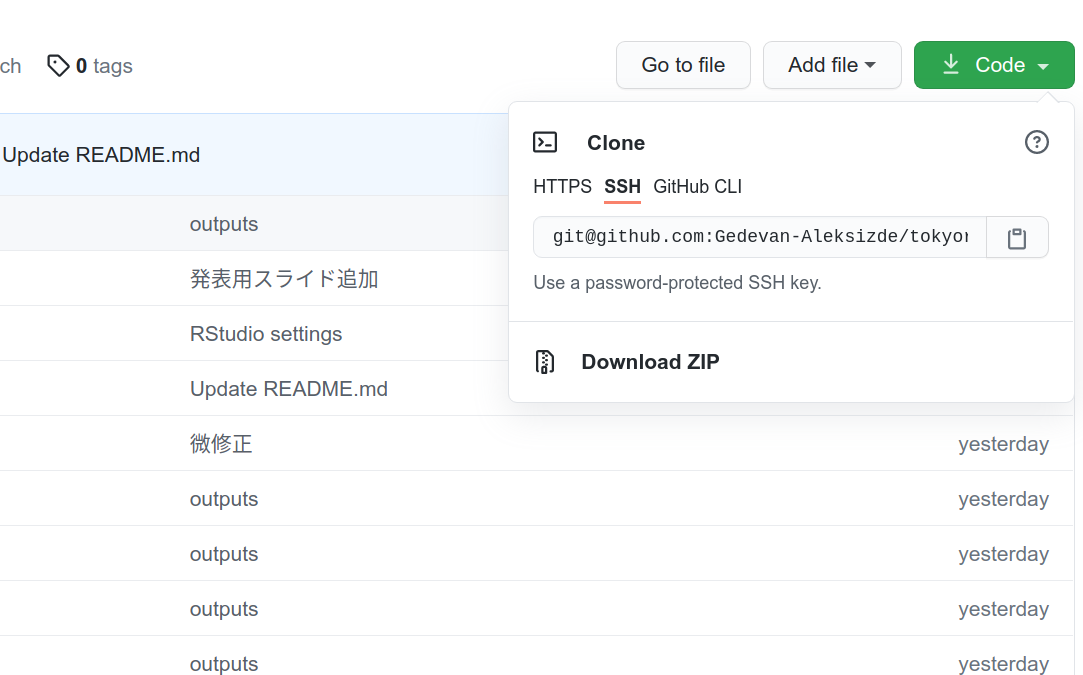
\includegraphics[width=1\linewidth,height=1\textheight,keepaspectratio]{img/github} \end{center}

\url{https://github.com/Gedevan-Aleksizde/tokyor-91-rmd}

なお, この文書も R Markdown で書かれており, 上記に含まれている \texttt{addendum.Rmd} から作成されています.

該当スクリプトファイルの中身をここにも転載しておきます. R のコマンド以外にもやることはあるので, ただコピペして実行するのではなく, 注意書きを読みながら実行してみてください. 特に, Mac と Linux ユーザの方は外部ライブラリのインストールが必要になりやすいと思います.

RStudio Cloud はおそらく Ubuntu を使用してるので, お使いの方は 「Ubuntu なら\ldots」「Linux なら\ldots」 と書いてある指示に従ってください.

\begin{Shaded}
\begin{Highlighting}[numbers=left,,]
\DocumentationTok{\#\#\#\#\# (1) RStudio のバージョンについて \#\#\#\#}
\CommentTok{\# 1.4.1103 は Windows 版では Python 使用時にエラーが発生します}
\CommentTok{\# もし Python を使いたいなら新しいバージョンが出るまで待つか,}
\CommentTok{\# 以下の daily build のどれかをインストールしてください}
\CommentTok{\# https://dailies.rstudio.com/rstudio/oss/windows/}

\DocumentationTok{\#\#\#\#\# (2) パッケージのインストール \#\#\#\#}
\CommentTok{\# インストール済みであっても最新版にしておいてください}
\CommentTok{\# ダイアログボックスでなにか言われたらNO!}
\FunctionTok{install.packages}\NormalTok{(}
  \FunctionTok{c}\NormalTok{(}
    \StringTok{"tidyverse"}\NormalTok{,}
    \StringTok{"remotes"}\NormalTok{,}
    \StringTok{"rmarkdown"}\NormalTok{,}
    \StringTok{"bookdown"}\NormalTok{,}
    \StringTok{"officedown"}\NormalTok{,}
    \StringTok{"citr"}\NormalTok{,}
    \StringTok{"ymlthis"}\NormalTok{,}
    \StringTok{"svglite"}\NormalTok{,}
    \StringTok{"kableExtra"}
\NormalTok{  )}
\NormalTok{)}

\DocumentationTok{\#\#\#\#\# (3) ragg インストール \#\#\#\#}
\FunctionTok{install.packages}\NormalTok{(}\StringTok{"ragg"}\NormalTok{)}
\CommentTok{\# ragg のインストール時, Mac/Linux では追加で外部ライブラリのインストールが要求されることがあります.}
\CommentTok{\# その際は手動でインストールしてください. おそらくは以下のような操作になります.}
\CommentTok{\#}
\CommentTok{\# 例えば Ubuntu なら}
\CommentTok{\# sudo apt install libharfbuzz{-}dev libfribidi{-}dev}
\CommentTok{\#}
\CommentTok{\# Mac なら homebrew でインストールします}
\CommentTok{\# brew install harfbuzz fribidi}

\DocumentationTok{\#\#\#\#\# (4) PDF 画像の準備 \#\#\#\#}
\CommentTok{\# さらに PDF で画像を出力したい場合は, X11 と Cairo が必要です.}
\CommentTok{\# Windows の場合, 以下が TRUE になっていることを確認してください}
\FunctionTok{capabilities}\NormalTok{()[}\FunctionTok{c}\NormalTok{(}\StringTok{"cairo"}\NormalTok{)]}
\CommentTok{\# Mac や Linux の場合は, 両方が TRUE になっていることを確認してください.}
\FunctionTok{capabilities}\NormalTok{()[}\FunctionTok{c}\NormalTok{(}\StringTok{"X11"}\NormalTok{, }\StringTok{"cairo"}\NormalTok{)]}

\CommentTok{\# Windows や多くの Linux 系はあまり気にしなくても良いですが,}
\CommentTok{\# 最近の Mac はデフォルトで必要なプログラムが入っていないようです.}
\CommentTok{\# Mac は以下の2つをインストールすれば使えます (インストールには homebrew が必要です).}
\CommentTok{\# ただし, xquartz のほうはうまく行かない例が報告されています.}
\CommentTok{\# https://www.xquartz.org/ で dmg ファイルをダウンロードしてインストールすることも試してください.}
\CommentTok{\#}
\CommentTok{\# brew install cairo}
\CommentTok{\# brew cask install xquartz}

\DocumentationTok{\#\#\#\#\# (5) rmdja パッケージのインストール \#\#\#\#}
\CommentTok{\# PDF は設定が複雑なので, 私の作成した rmdja パッケージを使うことをお薦めします.}
\CommentTok{\# このセッション時点では最新版は v0.4.5 です}
\NormalTok{remotes}\SpecialCharTok{::}\FunctionTok{install\_github}\NormalTok{(}\StringTok{"Gedevan{-}Aleksizde/rmdja"}\NormalTok{, }\AttributeTok{upgrade =} \StringTok{"never"}\NormalTok{)}

\DocumentationTok{\#\#\#\#\# (6) TeX のインストールします \#\#\#\#}
\CommentTok{\# これはすでにインストールしている人, PDF 文書の作成を目的としていない人は不要です}
\CommentTok{\# それなりに時間がかかるので注意してください}
\NormalTok{tinytex}\SpecialCharTok{::}\FunctionTok{install\_tinytex}\NormalTok{()}
\NormalTok{tinytex}\SpecialCharTok{::}\FunctionTok{tlmgr\_install}\NormalTok{(}\StringTok{"texlive{-}msg{-}translations"}\NormalTok{)}

\DocumentationTok{\#\#\#\#\# (7) 共通フォントのインストール (Linux のみ) \#\#\#\#}
\CommentTok{\# 以降の説明を簡単にするため, Linux でのフォントを共通化します.}
\CommentTok{\# これは Linux 系 OS をお使いの方のみ必要です.}
\CommentTok{\# Linux 系 OS をお使いならば, Noto フォントをおすすめします.}
\CommentTok{\# 例えば Ubuntu (RStudio Cloud も Ubuntu OS です) ならば以下でインストールできます}
\CommentTok{\# sudo apt install fonts{-}noto{-}cjk fonts{-}noto{-}cjk{-}extra}


\CommentTok{\# {-}{-}{-}{-} ここで念の為 RStudio 再起動 {-}{-}{-}{-}}

\CommentTok{\# PDF の閲覧は okular が便利です. MS Store で入手できます}
\CommentTok{\# https://www.microsoft.com/ja{-}jp/p/okular/9n41msq1wnm8?rtc=1\&activetab=pivot:overviewtab}
\CommentTok{\#}
\CommentTok{\# Sumatra は軽量ですが, フォントの埋め込みを確認できません.}


\CommentTok{\# {-}{-}{-}{-}{-} 以下は基本チュートリアルの範囲ではあまり取り上げませんが, 便利な拡張パッケージです}

\CommentTok{\# Python 使いたい人へ}
\FunctionTok{install.package}\NormalTok{(}\StringTok{"reticulate"}\NormalTok{)}

\CommentTok{\# Julia 使いたい人へ}
\FunctionTok{install.package}\NormalTok{(}\StringTok{"JuliaCall"}\NormalTok{)}

\CommentTok{\# ragg が使えない/Linux 以外で PDF 形式の画像で文字化けを防ぎたい場合は以下を試してください.}
\NormalTok{remotes}\SpecialCharTok{::}\FunctionTok{install\_github}\NormalTok{(}\StringTok{"Gedevan{-}Aleksizde/fontregisterer"}\NormalTok{, }\AttributeTok{upgrade =} \StringTok{"never"}\NormalTok{)}

\FunctionTok{install.packages}\NormalTok{(}\FunctionTok{c}\NormalTok{(}
  \StringTok{"xaringan"}\NormalTok{,}
  \StringTok{"bookdownplus"}\NormalTok{,}
  \StringTok{"blogdown"}\NormalTok{,}
  \StringTok{"pagedown"}
\NormalTok{))}

\CommentTok{\# "word" 関連}
\FunctionTok{install.packages}\NormalTok{(}
  \FunctionTok{c}\NormalTok{(}
    \StringTok{"officer"}\NormalTok{, }\StringTok{"rvg"}\NormalTok{, }\StringTok{"openxlsx"}\NormalTok{,}
    \StringTok{"ggplot2"}\NormalTok{, }\StringTok{"flextable"}\NormalTok{, }\StringTok{"xtable"}\NormalTok{, }\StringTok{"rgl"}\NormalTok{, }\StringTok{"stargazer"}\NormalTok{,}
    \StringTok{"tikzDevice"}\NormalTok{, }\StringTok{"xml2"}\NormalTok{, }\StringTok{"broom"}
\NormalTok{  )}
\NormalTok{)}
\CommentTok{\# パワーポイントやWordにグラフをエクスポートする}
\NormalTok{remotes}\SpecialCharTok{::}\FunctionTok{install\_github}\NormalTok{(}\StringTok{"tomwenseleers/export"}\NormalTok{)}
\CommentTok{\# Word の更新差分を考慮して編集できる (ただし現在開発停止中)}
\NormalTok{remotes}\SpecialCharTok{::}\FunctionTok{install\_github}\NormalTok{(}\StringTok{"noamross/redoc"}\NormalTok{)}
\end{Highlighting}
\end{Shaded}

\begin{infobox}{important}
上記のインストール手順が難しくて分からないという方は, 少なくとも R Markdown で最低限のチュートリアル操作をするのに必要な \textbf{rmarkdown} と \textbf{bookdown} と \textbf{tinytex} がインストールされ, かつ \textbf{tinytex} で TeX をインストールできていることを確認してください. ただし, この場合はチュートリアルで紹介する機能の一部が使えない可能性があります.

\end{infobox}

\hypertarget{first-step}{%
\section{始めの一歩}\label{first-step}}

\hypertarget{ux6700ux521dux306eux6587ux66f8ux4f5cux6210}{%
\subsection{最初の文書作成}\label{ux6700ux521dux306eux6587ux66f8ux4f5cux6210}}

まずは文書を作成するまでをやってみましょう.

RStudio の左上のボタンを押し, R Markdown ファイルを新規作成します. 「R Markdown\ldots」がそれです.

\begin{center}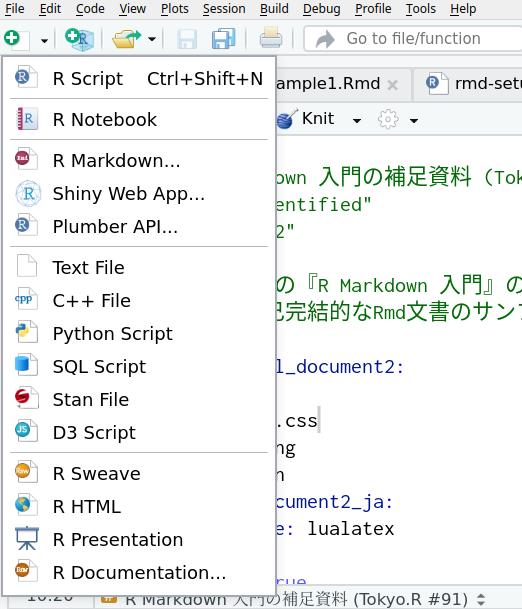
\includegraphics[width=1\linewidth,height=1\textheight,keepaspectratio]{img/newfile} \end{center}

ウィンドウが現れます. デフォルトでは左側は ``Documet,'' 右側のラジオボタンは ``HTML'' を選択しているはずです. このデフォルトの選択で決定してください.

\begin{center}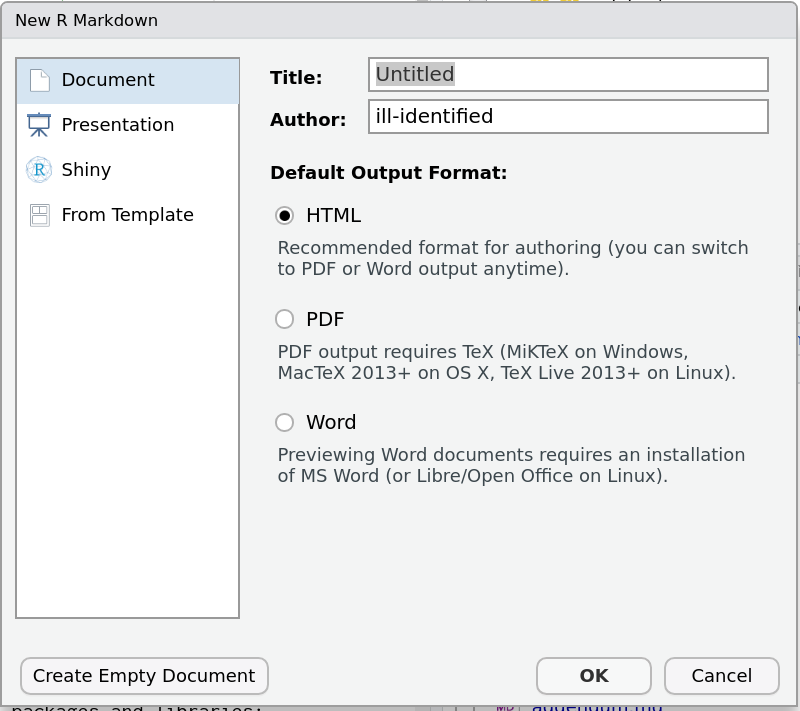
\includegraphics[width=1\linewidth,height=1\textheight,keepaspectratio]{img/select-html} \end{center}

新しい R Markdown ファイルが開かれます. すでに何か書かれているはずです. これは初心者のための出力サンプルです. これを適当な名前で保存してください. なお, R Markdown ファイルの拡張子は \texttt{.Rmd} です.

まずは文書のタイトルと著者を書き換えてみましょう. 冒頭の \texttt{-\/-\/-}, \texttt{-\/-\/-} で囲まれた部分を書き換えてみましょう. \texttt{title:}, \texttt{author:} の右側の部分です. タイトルは ``Untitled'', ユーザー名はおそらくあなたのPCアカウント名になっているでしょう.

\begin{center}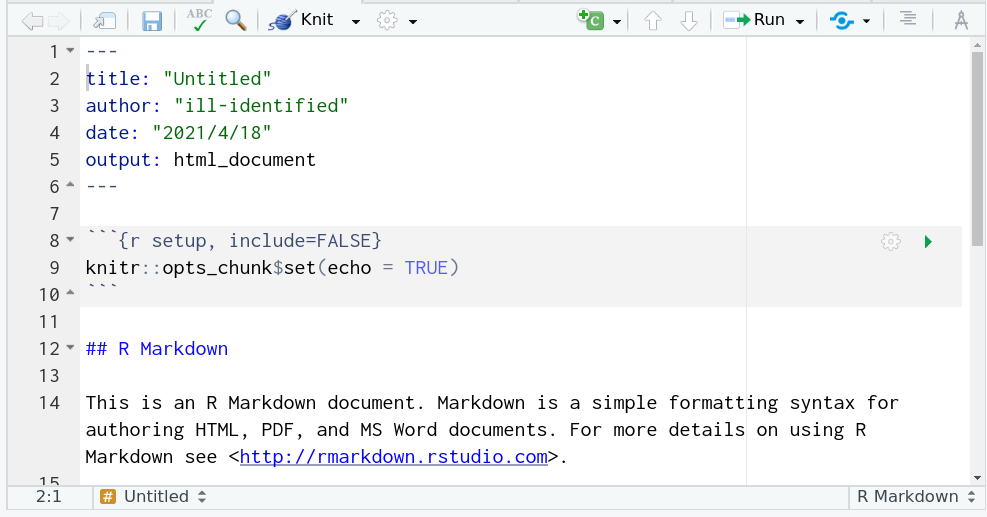
\includegraphics[width=1\linewidth,height=1\textheight,keepaspectratio]{img/newbie} \end{center}

これを以下のように書き換えてみましょう (他のタイトルや名前にしてもいいです.)

\begin{Shaded}
\begin{Highlighting}[]
\FunctionTok{title}\KeywordTok{:}\AttributeTok{ }\StringTok{"はじめての R Markdown"}
\FunctionTok{author}\KeywordTok{:}\AttributeTok{ }\StringTok{"Tokyo.R 太郎"}
\end{Highlighting}
\end{Shaded}

\begin{center}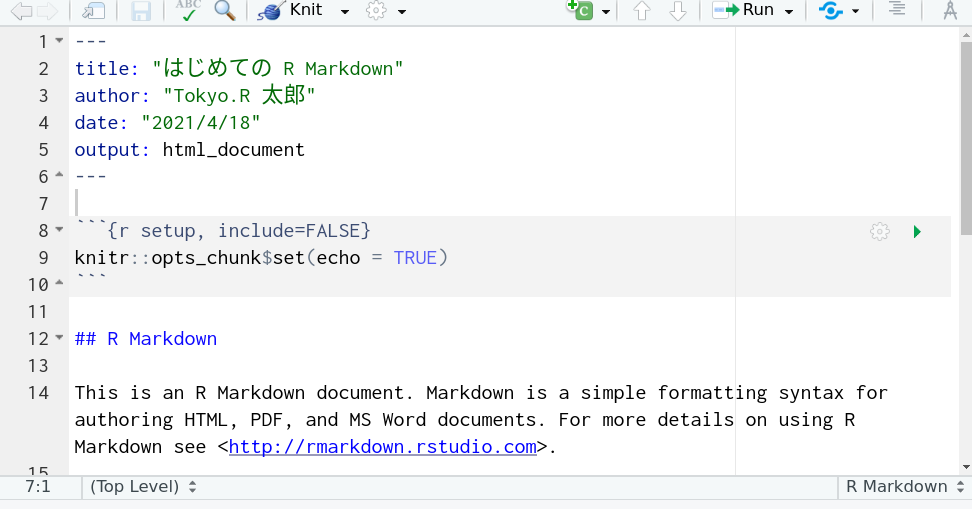
\includegraphics[width=1\linewidth,height=1\textheight,keepaspectratio]{img/newbie2} \end{center}

\begin{infobox}{important}
コロン (\texttt{:}) の後にはスペース1つ以上を空けることを忘れないでください

\end{infobox}

書き換えたら, 上記を一旦保存します. 名前は何でもいいです. 拡張子は自動的に \texttt{.Rmd} となるはずです.

では, Rmd ファイルから文書を生成させます. この処理を\textbf{コンパイル}といいます. 文書のコンパイルは, RStudio のエディタの上にある, \includegraphics{156470aaae9d104f8a7bb4e632e5d7401a34c744.png}ボタンを押します.

下のタブでなにやらログが流れた後, 新しいウィンドウに生成された HTML 文書が生成されるはずです. また, 同じフォルダに .Rmd の拡張子が .html となったファイルもできています.

\begin{center}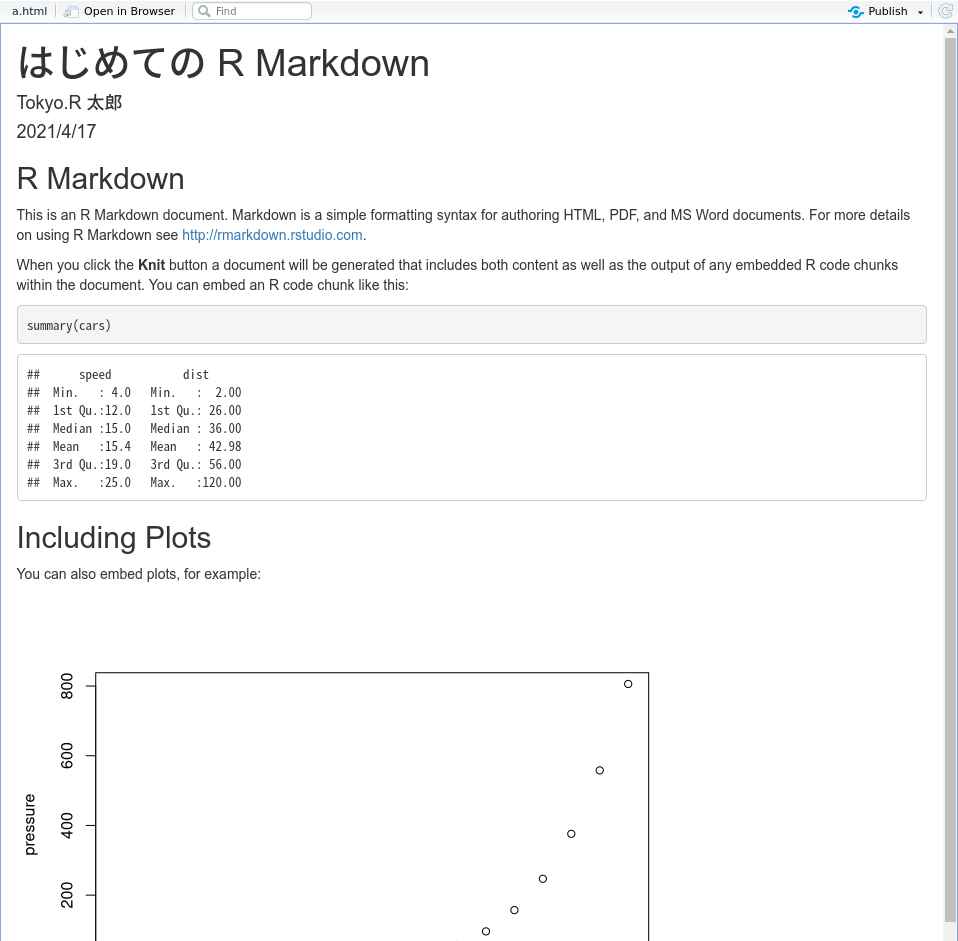
\includegraphics[width=1\linewidth,height=1\textheight,keepaspectratio]{img/plain-document} \end{center}

さて, これで初めての \textbf{R Markdown 文書の作成に成功}しました!

\begin{infobox}{important}
R Markdown では基本的に, \includegraphics{156470aaae9d104f8a7bb4e632e5d7401a34c744.png}ボタンを押すタイミングで Rmd ファイルの内容が反映されます.\footnote{例外は R Notebook です.} よって, Rmd ファイルの中身を書き換えた場合, \includegraphics{156470aaae9d104f8a7bb4e632e5d7401a34c744.png}ボタンを再度押さなければ内容が反映されません.

\end{infobox}

しかし, これだけでは R Markdown をレポート作成に活用できたとは言えません. というわけで, 以降では基本的な使い方を紹介していきます.

\hypertarget{markdown-ux672cux6587ux306eux66f8ux304dux65b9}{%
\section{Markdown: 本文の書き方}\label{markdown-ux672cux6587ux306eux66f8ux304dux65b9}}

\begin{infobox}{important}
デフォルトのサンプル文は英語です. とっつきにくいのでこれを翻訳\&微修正したバージョンを冒頭の資料に同梱しました. ファイル名は \href{https://github.com/Gedevan-Aleksizde/tokyor-91-rmd/blob/main/example1.Rmd}{\texttt{example1.Rmd}} です. \textbf{以降はこれをコピーしたものを使用してください}.

\end{infobox}

\begin{center}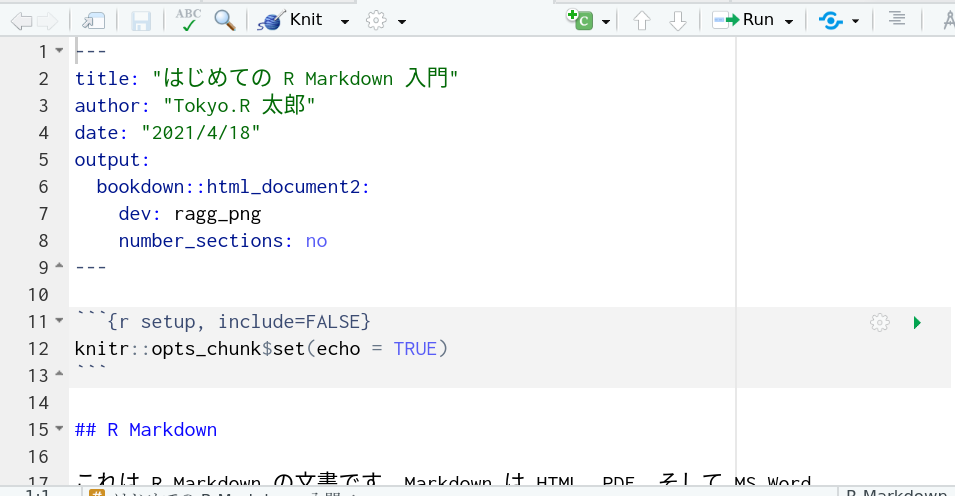
\includegraphics[width=1\linewidth,height=1\textheight,keepaspectratio]{img/example1-source} \end{center}

まずは R Markdown 上で本文を書く方法です. \texttt{-\/-\/-} 以下の部分は全て本文になります.

本文は Markdown と呼ばれる記法で書きます. これは HTML タグのようにプレーンテキストを装飾する記号ですが, \textbf{HTML タグよりシンプルで, 見やすいはずです}. ふだんメモ帳で書くような構文になることを意識されています.

最近は, Markdown は R に限らず様々なサービスで使われています. たとえばチャットツールの Slack の文字の装飾も Markdown で書くことができます.

以下に紹介する記法を, \texttt{example1.Rmd} 上でいろいろと試してみてください (ほとんどはデフォルトの \texttt{.Rmd} でも使えます).

\hypertarget{ux30c6ux30adux30b9ux30c8ux306eux88c5ux98fe}{%
\subsection{テキストの装飾}\label{ux30c6ux30adux30b9ux30c8ux306eux88c5ux98fe}}

\hypertarget{ux6587ux5b57ux306eux30b9ux30bfux30a4ux30ebux5909ux66f4}{%
\subsubsection{文字のスタイル変更}\label{ux6587ux5b57ux306eux30b9ux30bfux30a4ux30ebux5909ux66f4}}

文字の一部のスタイルを変更します. HTML でいえば \texttt{\textless{}span\textgreater{}} です.

文字の斜体/イタリックによる強調は, アスタリスク (\texttt{*}) で文字列を囲みます. \emph{このように表示されます}. そして太字は, アスタリスク2連続 (\texttt{**}) で囲みます. \textbf{このように表示されます}. この2つの記法は \texttt{*} だけでなく, アンダースコア \texttt{\_} でもできます.

また, プログラムの関数であることを強調したい場合はコード要素が良いでしょう. \textbf{バッククオート} (\texttt{\textasciigrave{}}, 日本語キーボードなら shift + \texttt{@} で入力できます) で囲みます. このように: \texttt{data.frame()}. なお, この方法でコードを書いても, \textbf{実行されるわけではありません}. 文書内でコードを実行する方法は, 後述のセクション\ref{code-chunk-practical}で紹介します.

\hypertarget{ux30cfux30a4ux30d1ux30fcux30eaux30f3ux30afux753bux50cfux306eux8cbcux308aux4ed8ux3051}{%
\subsubsection{ハイパーリンク・画像の貼り付け}\label{ux30cfux30a4ux30d1ux30fcux30eaux30f3ux30afux753bux50cfux306eux8cbcux308aux4ed8ux3051}}

ハイパーリンクは \texttt{{[}テキスト{]}(URL)} で書くことができます. このように \href{https://rpubs.com/ktgrstsh/755893}{Rpubs のこのページへのリダイレクト}ができます. 代替テキストが不要なら, URL をそのまま書き込んでもよいです: \url{https://rpubs.com/ktgrstsh/755893}.

まず, 画像ファイルの貼り付けは \texttt{!{[}代替テキスト{]}(画像のファイルパス)} のような構文です. つまりハイパーリンクの先頭に \texttt{!} が付いただけです.

\begin{verbatim}
![Tokyo.R](img/logo.png)
\end{verbatim}

\begin{figure}
\centering
\includegraphics[width=\textwidth,height=0.5\textheight]{3cb1243869ac5014588f744fdce5198d9a125278.png}
\caption{Tokyo.R}
\end{figure}

サイズの細かい指定やグラフの貼り付けは, 後述するコードチャンクを使う必要があります.

\hypertarget{ux4efbux610fux306eux4f4dux7f6eux3067ux6539ux884c}{%
\subsubsection{任意の位置で改行}\label{ux4efbux610fux306eux4f4dux7f6eux3067ux6539ux884c}}

ほとんどのワードプロセッサは自動で行を折り返してくれますが, 場合によっては手動で改行位置の調整が必要になります. しかし, Rmd ファイル上の改行は改行と認識されません. このような場合, \textbf{行末にスペース2つを追加}すると強制改行されます.

Rmd ファイルに以下のように書くと\ldots{}

\begin{verbatim}
**行の末尾にスペースを2つ**追加すると改行できます.  
(ここで改行されているはずです)このように
\end{verbatim}

こうなるはずです.

\textbf{行の末尾にスペースを2つ}追加すると改行できます.\\
(ここで改行されているはずです)このように

スペースの有無はわかりにくいですが, 実際に試してみればわかるはずです.

また, 空白行を1つ挟んでも改行されますが, 正確にはこれは行を改めているのではなく\textbf{段落}を改めています. これはブロック要素といいます.

\hypertarget{ux30d6ux30edux30c3ux30afux8981ux7d20}{%
\subsection{ブロック要素}\label{ux30d6ux30edux30c3ux30afux8981ux7d20}}

文中の一部ではなく, 独立した文のまとまりを定義することもできます. これらをまとめてブロック要素と呼びます (逆にさっきのようなものは「\textbf{インライン要素}」と呼びます). ブロックとは段落 (パラグラフ) のようなものです.

もっとも基本的なブロック要素は, まさに\textbf{段落の区切り}です\footnote{HTMLでは, 日本語文書のルールである「1文字下げ」は用意されていませんので, 見た目の変化としてはすこし空白が広い程度のものとなります.}. 1行以上の空白行をはさむと, それが段落の区切りとなります. それ以外のブロック要素も全て, 改行がブロックの単位を決めることになります. この文章はこの次に空白行を挟んでいるので, 段落が変わります.

ここからは新しい段落です.

\begin{infobox}{important}
ブロック要素の共通点として, \textbf{前後を空白の行で1行以上空け}なければブロック要素として認識されません.

\end{infobox}

\hypertarget{ux898bux51faux3057ux3092ux66f8ux304f}{%
\subsubsection{見出しを書く}\label{ux898bux51faux3057ux3092ux66f8ux304f}}

この資料のように, 見出しを付けたい場合は 行の先頭に \texttt{\#} を付け, その直後に\textbf{スペースを1つ空け}て書きます.

Rmd 上でこのように書きます.

\begin{verbatim}
# イントロダクション

本文

# 次のセクション

本文
\end{verbatim}

\texttt{\#} を増やし, \texttt{\#\#}, \texttt{\#\#\#} と書くと見出しの階層が下がっていきます. これは HTML の \texttt{\textless{}h2\textgreater{}}, \texttt{\textless{}h3\textgreater{}}, \ldots{} と同様です.

\hypertarget{ux7b87ux6761ux66f8ux304d}{%
\subsubsection{箇条書き}\label{ux7b87ux6761ux66f8ux304d}}

箇条書きをしたい場合は, アスタリスク \texttt{*} を先頭に付けます. 強調と区別するため, これも直後に\textbf{スペースを1つ空け}て書きます.

Rmd 上でこう書いたとします.

\begin{verbatim}
* 箇条書き
    * 一段下げた箇条書き
* 箇条書き
\end{verbatim}

それがこう表示されます.

\begin{itemize}
\tightlist
\item
  箇条書き

  \begin{itemize}
  \tightlist
  \item
    一段下げた箇条書き
  \end{itemize}
\item
  箇条書き
\end{itemize}

箇条書き記号は \texttt{*} の代わりにハイフン (\texttt{-}) やプラス (\texttt{+}) で書いても同様に使えます.

数字付きの箇条書きは, \texttt{1.} のように数字の後にドット (\texttt{.}) を付けます.\footnote{アルファベット順にすることもできますが, これは出力形式によっては機能しないことがあります.} これは文字通り \texttt{1.} と書き続けても\textbf{勝手に数字をカウントしてくれる}ので便利です. 逆に, 1 以外の数字を書くことでカウントを操作することもできます.

Rmd 上でこう書いたとします.

\begin{verbatim}
1. その1
    1. 一段下げたその1
1. その2
1. その3
\end{verbatim}

それがこう表示されます.

\begin{enumerate}
\def\labelenumi{\arabic{enumi}.}
\tightlist
\item
  その1

  \begin{enumerate}
  \def\labelenumii{\arabic{enumii}.}
  \tightlist
  \item
    一段下げたその1
  \end{enumerate}
\item
  その2
\item
  その3
\end{enumerate}

\hypertarget{ux30b3ux30fcux30c9ux30d6ux30edux30c3ux30af}{%
\subsubsection{コードブロック}\label{ux30b3ux30fcux30c9ux30d6ux30edux30c3ux30af}}

インライン要素のコードの強調 \texttt{\textasciigrave{}} は, 長いコードの表示に不向きです.

\texttt{data(mtcars)}~\\
\texttt{fit\ \textless{}-\ lm(mpg\ \textasciitilde{}.,\ data\ =\ mpg)}~\\
\texttt{summary(fit)}

このように見づらく, 1行ごとにバッククオートや改行構文を書かねばなりません. 複数行にわたるコードを書く場合は, インラインのコード強調ではなく, ブロック要素のコード強調, コードブロックを使います. コードブロックはバッククオート3連続 (\texttt{\textasciigrave{}\textasciigrave{}\textasciigrave{}}) で囲んだ部分です. この内部では改行もそのまま表示されます.

Rmd ファイル上では以下のように書きます.

\begin{verbatim}
```
data(mtcars)
fit <- lm(mpg ~., data = mpg)
summary(fit)
```
\end{verbatim}

これが実際にはこう表示されます.

\begin{verbatim}
data(mtcars)
fit <- lm(mpg ~., data = mpg)
summary(fit)
\end{verbatim}

なお, R コードの埋め込みは\textbf{この方法ではできません}. これはコードの表示のみです. 中身を実行したい場合は, この次のコードチャンクのセクションを見てください

\hypertarget{code-chunk-init}{%
\subsubsection{コードチャンク (第一歩)}\label{code-chunk-init}}

コードブロックはコードを掲載するだけで, 実行はできませんでした. 実行する機能があるのは\textbf{コードチャンク}で, これが R Markdown を使う大きなメリットの1つです.

コードチャンクの書き方はコードブロックと似ていますが, R として実行することを意味するため, \texttt{\textasciigrave{}\textasciigrave{}\textasciigrave{}} の後にさらに \texttt{\{r\}} を付けます. 以下は \texttt{example1.Rmd} にも含まれているコードチャンクです.

\begin{verbatim}
```{r}
summary(cars)
```
\end{verbatim}

すると, 以下のように表示されます.

\begin{Shaded}
\begin{Highlighting}[numbers=left,,]
\FunctionTok{summary}\NormalTok{(cars)}
\end{Highlighting}
\end{Shaded}

\begin{verbatim}
##      speed           dist       
##  Min.   : 4.0   Min.   :  2.00  
##  1st Qu.:12.0   1st Qu.: 26.00  
##  Median :15.0   Median : 36.00  
##  Mean   :15.4   Mean   : 42.98  
##  3rd Qu.:19.0   3rd Qu.: 56.00  
##  Max.   :25.0   Max.   :120.00
\end{verbatim}

また, グラフも表示されます.

\begin{center}\includegraphics[width=1\linewidth,height=1\textheight,keepaspectratio]{addendum_files/figure-latex/pressure-1} \end{center}

ふだん R で見ているものと全く同じものが出力できました. しかし, あなたが作りたいレポートは, \textbf{プログラム部分の表示が不要}だったり, コードのみだったり, \textbf{作成したグラフや, データフレームをかっこよく整形した表}だったりするかもしれません. それらも\textbf{全て可能}です. コードチャンクでできることは多彩ですが, その説明は一旦, セクション\ref{code-chunk-practical}に後回しにします.

\hypertarget{ux30d3ux30b8ux30e5ux30a2ux30ebux30a8ux30c7ux30a3ux30bf}{%
\subsection{ビジュアルエディタ}\label{ux30d3ux30b8ux30e5ux30a2ux30ebux30a8ux30c7ux30a3ux30bf}}

Markdown はこのように便利ですが, プレーンテキストで書くのがどうしても苦手という場合は, \textbf{ビジュアル Markdown エディタ}という Word 風のエディタがあります. これは RStudio 1.4以降で提供されるようになりました.

右上のコンパスのようなアイコン\includegraphics{3fa0e102526db03f68cc8a22bb92e1a0926c4f5f.png}をクリックしてください.

\begin{center}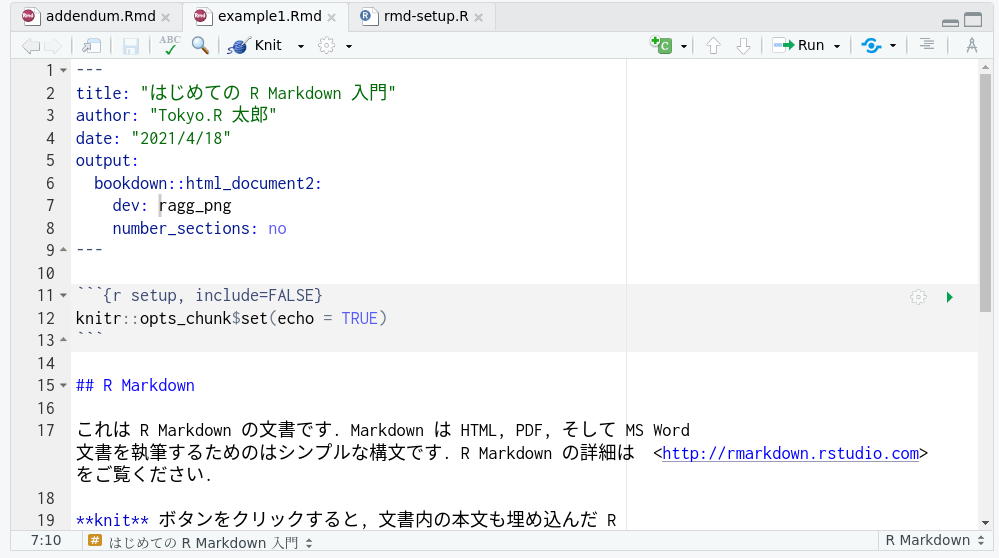
\includegraphics[width=1\linewidth,height=1\textheight,keepaspectratio]{img/vme-button} \end{center}

すると, 以下のような Word 風の画面になります. フォントスタイルやいろいろな項目の画像の挿入がツールバーから行えるようになっています.

\begin{center}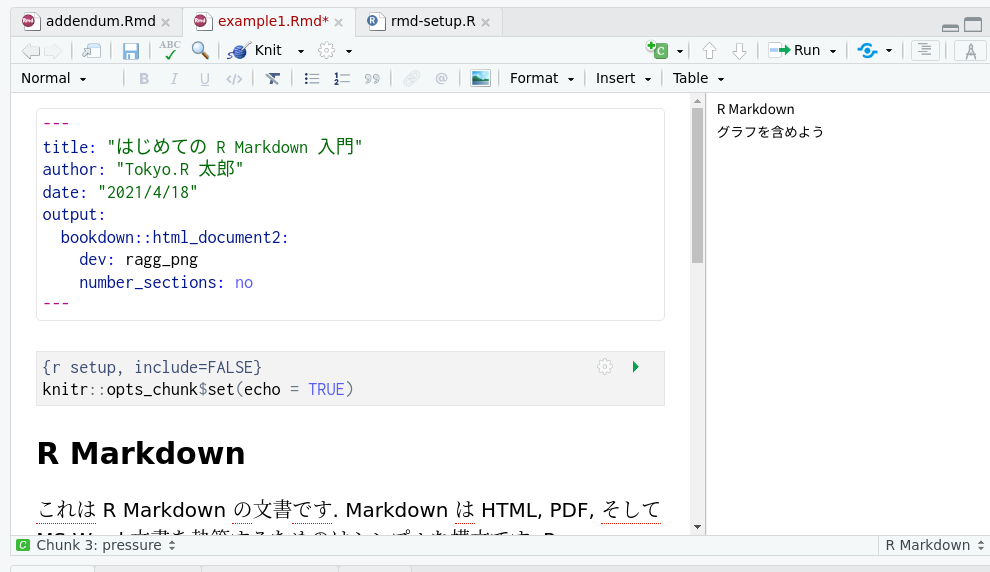
\includegraphics[width=1\linewidth,height=1\textheight,keepaspectratio]{img/visual-editor2} \end{center}

\begin{center}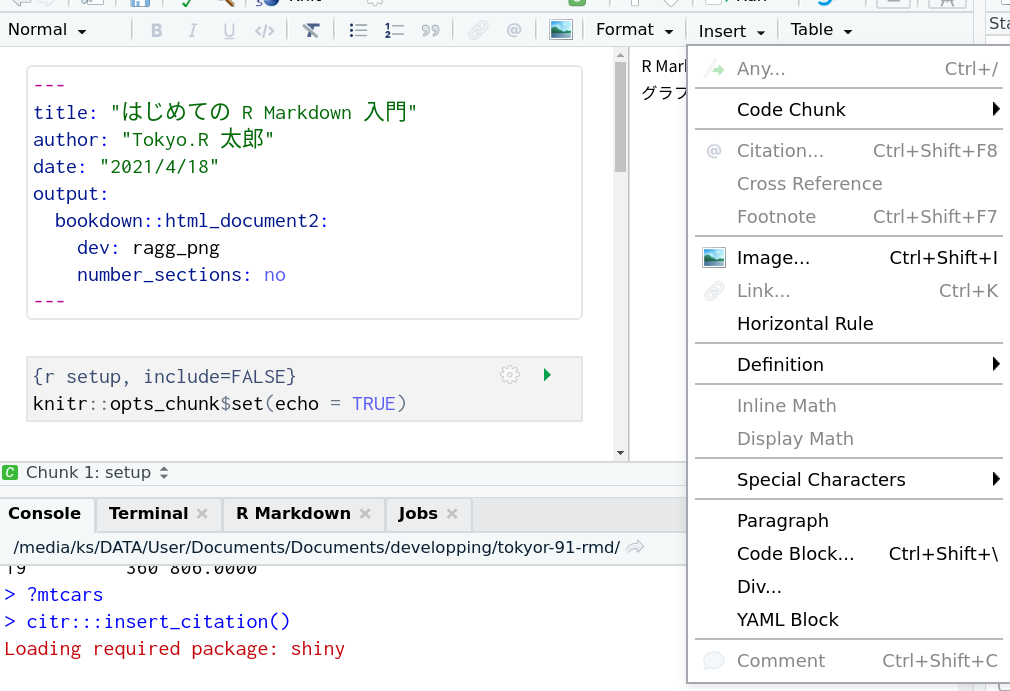
\includegraphics[width=1\linewidth,height=1\textheight,keepaspectratio]{img/visual-editor1} \end{center}

ただし, ここでは出力が HTML なので, RStudio 上の見た目と全く同じ文書が生成されるわけではないことに注意してください. 他の媒体でも同様です.

ビジュアルエディタをやめて通常のエディタに戻したい場合は, コンパスのボタンを再度クリックしてください. 右側に目次 (アウトライン) の表示が残ったままかもしれません. \includegraphics{3fa0e102526db03f68cc8a22bb92e1a0926c4f5f.png} の左隣にある\includegraphics{c5f662c3bca3ef24370bba579eb35d1a9af7f3b5.png} アイコンが, アウトラインの表示・非表示を切り替えるボタンです. Markdown の構文を覚えられてないうちは, これで構文の使い方を真似るとよいかもしれません.

これは個人的な意見ではありますが, Markdown 構文はとてもシンプルで効率的に書けますので, R Markdown をよく使う予定ならばなるべく早めに Markdown を覚え, ビジュアルエディタモードを卒業することをおすすめします.

\begin{infobox}{important}
ビジュアルエディタはファイルを自動で整形するため, 通常のエディタと何度も切り替えると不具合を起こす可能性があります. 1つのファイルに対して, どちらか1つのモードしか使わないことをお薦めします.

\end{infobox}

\hypertarget{outputs}{%
\section{出力文書の変更}\label{outputs}}

先ほどのチュートリアルでは HTML 文書を作成しました. しかしみなさんがほしいのは Word かもしれませんし, PDF かもしれません. \textbf{rmarkdown} パッケージは以下をサポートしています.

\begin{itemize}
\tightlist
\item
  HTML (より詳しく言うと, Bootstrap3 ベース)
\item
  PDF (LaTeX を利用)
\item
  MS Word (当然ですが DOCX 形式のみです)
\end{itemize}

さらに, プレゼン用スライドなど, 体裁に応じたスタイル変更もできます.

この出力の変更は, 再び冒頭の設定を書き換えることで実現できます.

\hypertarget{ux51faux529bux30d5ux30a9ux30fcux30deux30c3ux30c8}{%
\subsection{出力フォーマット}\label{ux51faux529bux30d5ux30a9ux30fcux30deux30c3ux30c8}}

デフォルトの文書では, 冒頭に

\begin{verbatim}
title: "..."
author: "..."
date: "..."
output: html_document
\end{verbatim}

と書かれていました. また, 今回提供している \texttt{example1.Rmd} には

\begin{verbatim}
output:
  bookdown::html_document2:
    dev: ragg_png
    number_sections: no
\end{verbatim}

と書かれています. この \texttt{output:} という項目が, 文書の出力を決めるもっとも重要な部分です. ここに指定されているものを, \textbf{出力フォーマット関数}または単に\textbf{出力フォーマット}といいます.

\textbf{rmarmkdown} パッケージには, 例えば以下のような出力フォーマットが用意されています.

\begin{itemize}
\tightlist
\item
  \texttt{html\_document}: HTML 文書
\item
  \texttt{html\_notebook}: Notebook 文書, リアルタイムで更新される
\item
  \texttt{pdf\_document}: PDF 文書
\item
  \texttt{word\_document}: Word (DOCX) 文書
\item
  \texttt{slidy\_presentation}: HTML 形式のスライド
\item
  \texttt{beamer\_presentation}: PDF 形式のスライド
\end{itemize}

「出力フォーマット関数」という名前が示すように, 実態は R の関数です. 細かい仕様は関数のヘルプとして見ることができます.

では, 試しに DOCX 形式にしてみましょう. Word がインストールされていなくても変換できますし, 閲覧には Libre Office などが使えます\footnote{ただし, Libre Office では表示が完全でないことがあります}.

\texttt{example1.Rmd} の冒頭の

\begin{Shaded}
\begin{Highlighting}[]
\FunctionTok{output}\KeywordTok{:}
\AttributeTok{  bookdown:}\FunctionTok{:html\_document2}\KeywordTok{:}
\AttributeTok{    }\FunctionTok{dev}\KeywordTok{:}\AttributeTok{ ragg\_png}
\AttributeTok{    }\FunctionTok{number\_sections}\KeywordTok{:}\AttributeTok{ }\CharTok{no}
\end{Highlighting}
\end{Shaded}

の \texttt{output:} 以下の行を, このように書き換えて保存します (複数行あります. 消し忘れがないように).

\begin{Shaded}
\begin{Highlighting}[]
\FunctionTok{output}\KeywordTok{:}\AttributeTok{ word\_document}
\end{Highlighting}
\end{Shaded}

そして \includegraphics{156470aaae9d104f8a7bb4e632e5d7401a34c744.png} します. \texttt{.docx} ファイルが作成されるはずです (お使いの環境によりますが, 今回は自動で開かれないかもしれません).

なお, Word (\texttt{word\_document}) や パワーポイント (\texttt{powerpoint\_presentation}) などの Office 系出力フォーマットは, HTML や PDF と比べて細部のスタイルが崩れやすい傾向にあります\footnote{これは内部で使用している Pandoc などの影響もあります. 新しいバージョンの Pandoc を使用したり, パッケージの開発版を使用することで改善されることもあります. しかしそれは「入門チュートリアル」の範疇を超えるためここには書きません.}. しかし PDF や HTML と違い DOCX や PPTX は編集用ファイルなので, 編集が容易です. よって手動で調整する想定になっています.

開くとエクスポートされているはずです (以下は Libre Office で開いた場合です).

\begin{center}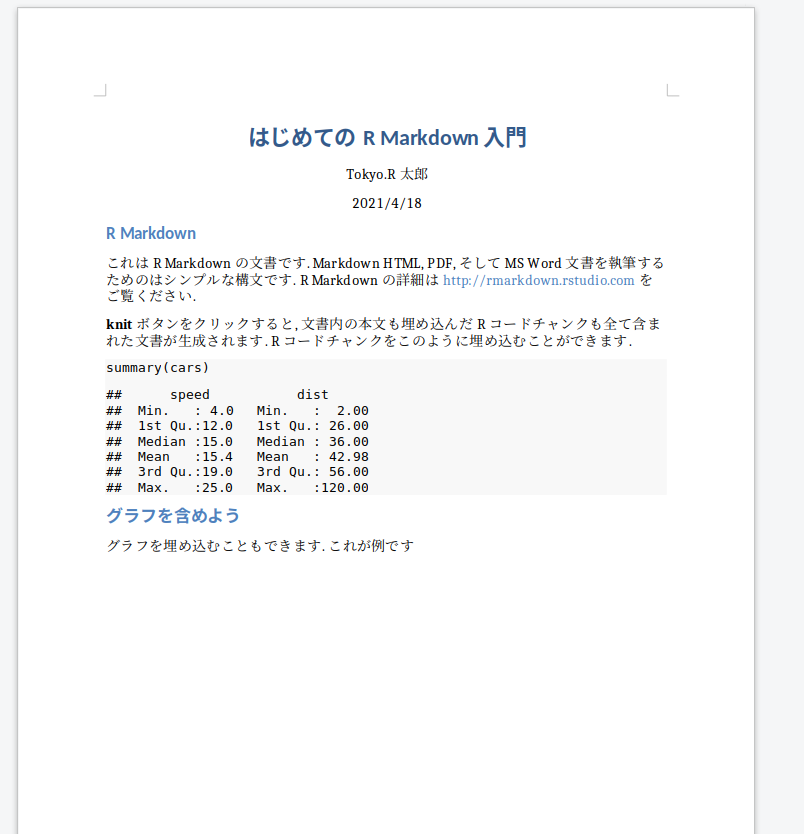
\includegraphics[width=1\linewidth,height=1\textheight,keepaspectratio]{img/example1-word} \end{center}

では PDF はどうでしょうか. ここまでの流れから, 以下のようにすれば良さそうです.

\begin{Shaded}
\begin{Highlighting}[]
\FunctionTok{outout}\KeywordTok{:}\AttributeTok{ pdf\_document}
\end{Highlighting}
\end{Shaded}

しかし, 実際にはなにかよくわからないエラーが表示され, うまくいかないか, うまく表示されないと思います. とりあえず出力したい場合は,

\begin{Shaded}
\begin{Highlighting}[]
\FunctionTok{output}\KeywordTok{:}\AttributeTok{ rmdja::pdf\_document2\_ja}
\end{Highlighting}
\end{Shaded}

とすれば動くでしょう.

\begin{infobox}{important}
今回の入門で初めて TeX をインストールした場合, PDF の初回コンパイルには時間がかかるかもしれません.

\end{infobox}

これは見ての通り \textbf{rmdja} パッケージを利用しています. もしインストールしていないのなら, YAML メタデータに次のような設定をすることで, \textbf{rmarkdown} のみで一応は日本語を表示することができます.

\begin{Shaded}
\begin{Highlighting}[]
\FunctionTok{output}\KeywordTok{:}
\AttributeTok{  }\FunctionTok{pdf\_document}\KeywordTok{:}
\AttributeTok{    }\FunctionTok{latex\_engine}\KeywordTok{:}\AttributeTok{ lualatex}
\FunctionTok{documentclass}\KeywordTok{:}\AttributeTok{ ltjsarticle}
\FunctionTok{classoption}\KeywordTok{:}\AttributeTok{ haranoaji}
\end{Highlighting}
\end{Shaded}

しかし, 平文のみのテキストなど簡単な文書ならよいですが, いろいろ使っているうちに問題が出てくるとおもいます. 日本語 PDF をうまく出力するにはいろいろな設定が必要になるためです. PDF 出力のカスタマイズはかなり複雑です. それはセクション\ref{pdf-intro}で紹介します.

スライドもフォーマットの書き換えで作成できますが, いくつか注意点があります. しかしそれは後のセクション\ref{slides}で紹介します.

\hypertarget{ux5404ux7a2eux30d5ux30a9ux30fcux30deux30c3ux30c8}{%
\subsection{各種フォーマット}\label{ux5404ux7a2eux30d5ux30a9ux30fcux30deux30c3ux30c8}}

他にもいろいろなパッケージがカスタマイズされた出力フォーマットを提供しています(表\ref{tab:format-tab}). 2021/4/17 時点では, 以下がおすすめです. 冒頭の環境設定ができていれば, 必要パッケージは全て入っているはずです.

\begin{table}

\caption{\label{tab:format-tab}主な出力フォーマット}
\centering
\begin{tabular}{ll}
\toprule
ファイル形式 & フォーマット関数名\\
\midrule
PDF & `rmdja::pdf\_document2\_ja`\\
HTML & `bookdown::html\_document2`\\
Word (DOCX) & `officedown::rdocx\_document`\\
スライド資料 (PDF) & `rmdja::beamer\_presentation\_ja`\\
スライド資料 (HTML) & `xaringan::tsukuyomi`\\
\addlinespace
スライド資料 (PPTX) & `officedown::rpptx\_document`\\
\bottomrule
\end{tabular}
\end{table}

\textbf{rmarkdown} 本体の出力フォーマットが1つもありませんが, それは次のような理由です.

\begin{itemize}
\tightlist
\item
  デフォルトのフォーマットに対して, \textbf{bookdown} の \texttt{...2} というフォーマットは相互参照機能が追加されている
\item
  PDF 形式のフォーマットはどれも, 日本語の文書として自然な形にするために必要な設定項目が多すぎる
\item
  \textbf{officedown} パッケージは, Word や PowerPoint のデフォルトの形式にスタイルの適用機能などが追加されている
\item
  \textbf{xaringan} パッケージは, より便利な構文が追加されている
\end{itemize}

\hypertarget{output-ux30d5ux30a3ux30fcux30ebux30c9ux306eux7de8ux96c6ux306bux3064ux3044ux3066}{%
\subsection{\texorpdfstring{\texttt{output} フィールドの編集について}{output フィールドの編集について}}\label{output-ux30d5ux30a3ux30fcux30ebux30c9ux306eux7de8ux96c6ux306bux3064ux3044ux3066}}

Rmd ファイルの冒頭の \texttt{-\/-\/-} で囲まれた部分は \ruby[g]{YAML}{ヤメル} メタデータといい, 文書の出力を決めるいろいろな設定項目があります. しかし, チュートリアルの範囲ではほぼ \texttt{title}, \texttt{author}, \texttt{output} しか使いません. YAML メタデータでできることは多いですが, \texttt{output} が特に重要なので, 基本チュートリアルではここだけ解説します. YAML メタデータの詳細はセクション\ref{YAML}で独立して解説します.

\texttt{output} にはこのように出力フォーマットを指定できます. そして出力フォーマットは R の関数なので, さまざまなオプションを与えることができます. \texttt{example1.Rmd} の

\begin{Shaded}
\begin{Highlighting}[]
\FunctionTok{output}\KeywordTok{:}
\AttributeTok{  bookdown:}\FunctionTok{:html\_document2}\KeywordTok{:}
\AttributeTok{    }\FunctionTok{dev}\KeywordTok{:}\AttributeTok{ ragg\_png}
\AttributeTok{    }\FunctionTok{number\_sections}\KeywordTok{:}\AttributeTok{ }\CharTok{no}
\end{Highlighting}
\end{Shaded}

にある, \texttt{number\_sections:\ no} というのは実は出力フォーマット \texttt{bookdown::html\_document2()} に引数 \texttt{number\_sections\ =\ FALSE} を与えているのと同じです. YAML メタデータの構文では, オプションを与える場合はこのように, 以下のような書き方のルールがあります.

\begin{enumerate}
\def\labelenumi{\arabic{enumi}.}
\tightlist
\item
  \texttt{output:} の直後に改行
\item
  インデントしてから出力フォーマット関数を書く
\item
  出力フォーマット関数の後にも \texttt{:} を与える
\item
  さらに改行\&インデントしてからオプション引数を書く
\item
  オプション引数も \texttt{=} ではなく \texttt{:} で代入する
\end{enumerate}

特に, \textbf{YAML メタデータはインデントを揃えることが重要}です. R ではインデントをほとんど気にしないので, 初心者はここでよく失敗します.

よって, 複数のオプションを与える場合は例えば以下のように書き連ねることになります (以下で使われているオプションの意味はここでは解説しません. ヘルプなどを参照してください).

\begin{Shaded}
\begin{Highlighting}[]
\FunctionTok{output}\KeywordTok{:}
\AttributeTok{  bookdown:}\FunctionTok{:html\_document2}\KeywordTok{:}
\AttributeTok{    }\FunctionTok{number\_sections}\KeywordTok{:}\AttributeTok{ }\CharTok{no}
\AttributeTok{    }\FunctionTok{toc}\KeywordTok{:}\AttributeTok{ }\CharTok{no}
\AttributeTok{    }\FunctionTok{code\_folding}\KeywordTok{:}\AttributeTok{ show}
\AttributeTok{    }\FunctionTok{dev}\KeywordTok{:}\AttributeTok{ ragg\_png}
\end{Highlighting}
\end{Shaded}

さらに, 複数のフォーマットも指定できます.

\begin{Shaded}
\begin{Highlighting}[]
\FunctionTok{output}\KeywordTok{:}
\AttributeTok{  officedown:}\FunctionTok{:rdocx\_document}\KeywordTok{:}\AttributeTok{ default}
\AttributeTok{  bookdown:}\FunctionTok{:html\_document2}\KeywordTok{:}
\AttributeTok{    }\FunctionTok{number\_sections}\KeywordTok{:}\AttributeTok{ }\CharTok{no}
\AttributeTok{    }\FunctionTok{toc}\KeywordTok{:}\AttributeTok{ }\CharTok{no}
\AttributeTok{    }\FunctionTok{code\_folding}\KeywordTok{:}\AttributeTok{ show}
\AttributeTok{    }\FunctionTok{dev}\KeywordTok{:}\AttributeTok{ ragg\_png}
\end{Highlighting}
\end{Shaded}

その場合, \includegraphics{156470aaae9d104f8a7bb4e632e5d7401a34c744.png}で作成されるのは一番上のフォーマットのみです. \includegraphics{156470aaae9d104f8a7bb4e632e5d7401a34c744.png}ボタンの横の三角形のボタンを押すことで, 2番目以降のフォーマットを選択できます.

\begin{infobox}{important}
R Markdown には便利な出力フォーマットが多数存在し, また上記のように複数のフォーマットを指定できますが, 現状は1つの Rmd ファイルからHTML, PDF, DOCX など異なるファイルタイプでそれぞれ同じような出力を実現することはかなり困難を伴います. 特に, Word は特殊です. 熟練しないうちは, Rmd ファイル1つに対してどれか1種類だけを生成する用途に使うと良いでしょう.

\end{infobox}

\hypertarget{r-markdown-ux30c6ux30f3ux30d7ux30ecux30fcux30c8}{%
\subsection{R Markdown テンプレート}\label{r-markdown-ux30c6ux30f3ux30d7ux30ecux30fcux30c8}}

\textbf{rmarkdown} を含むいくつかのパッケージには, いろいろな項目を設定済みのテンプレートを提供しています. 新規作成のとき, 左側の ``From Templates'' を選ぶと, 右側にテンプレートの名称と, 提供元のパッケージ名が表示されます.

\begin{center}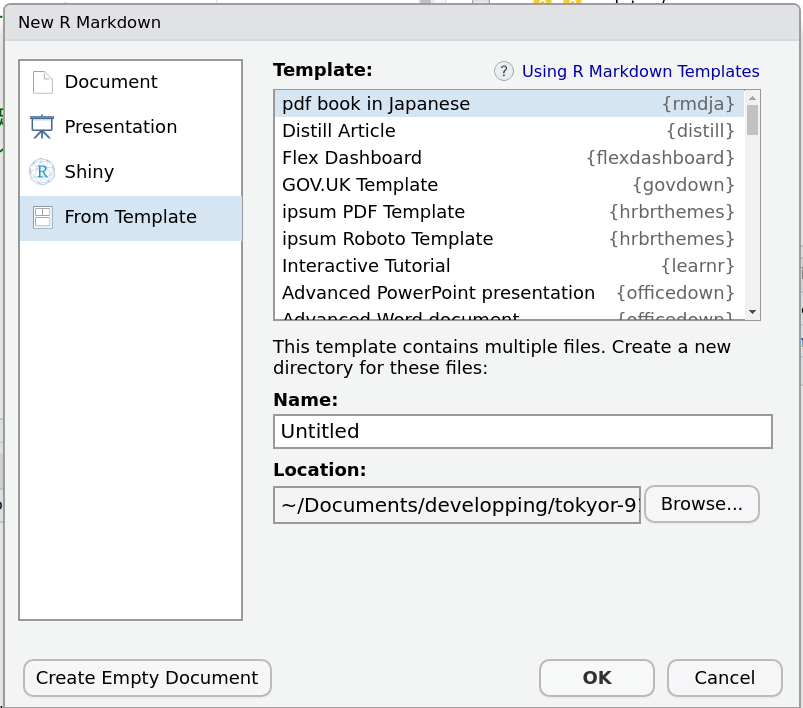
\includegraphics[width=1\linewidth,height=1\textheight,keepaspectratio]{img/templates} \end{center}

\hypertarget{code-chunk-practical}{%
\section{コードチャンクを使いこなす}\label{code-chunk-practical}}

セクション\ref{code-chunk-init}ではコードチャンクの最低限の使い方のみ紹介しましたが, 常にコードとテキストを出力するだけでは使いにくいと思います. そこで, より実用的な使い方を紹介します.

\hypertarget{ux30c1ux30e3ux30f3ux30afux30d8ux30c3ux30c0ux306bux3088ux308bux30abux30b9ux30bfux30deux30a4ux30ba}{%
\subsection{チャンクヘッダによるカスタマイズ}\label{ux30c1ux30e3ux30f3ux30afux30d8ux30c3ux30c0ux306bux3088ux308bux30abux30b9ux30bfux30deux30a4ux30ba}}

コードチャンクの先頭にある \texttt{\{r\}} は, \textbf{チャンクヘッダ}といい, 括弧内にそのチャンクの設定をいろいろと書き加えることができます.

基本的な書き方は以下です.

\begin{verbatim}
{r LABEL, echo = F, eval = T, ...}
\end{verbatim}

先頭の \texttt{r} は R 言語での実行を意味するため, 必須です. 次の \texttt{LABEL} は\textbf{チャンクラベル}といい, このチャンクの名前です. 好きな文字列を書けます. しかし, チャンクの識別のために\textbf{名前が重複しないように}してください. ほとんどの場合は, 後述する相互参照の時に使います. それ以外では省略してもかまいませんが, エラーが出た時にチャンクラベルを決めていると発生箇所が分かりやすいです. それ以降に\textbf{チャンクオプション} を追加できます. \textbf{R の関数の引数と同様に}, 必ずカンマ (\texttt{,}) で区切ってください. R の関数の引数というのがポイントで, ここには R の引数と同じように文字列は引用符で囲む必要があったり, R のコードを与えたりすることもできます.

代表的なチャンクオプションの使い方に, 以下があります.

\begin{itemize}
\tightlist
\item
  \texttt{echo\ =\ F}: コードを表示しない, スライドでは邪魔なのでよく非表示にします
\item
  \texttt{eval\ =\ F}: コードを実行しない, コードだけ見せたい時に
\item
  \texttt{fig.cap=""}: 図のキャプション
\item
  \texttt{fig.align\ =\ "center"}: 図を中央揃えにする (出力フォーマットでも一括設定できることがあります)
\end{itemize}

例えばサンプルには以下のようなチャンクがあります.

\begin{verbatim}
```{r pressure, echo = F}
plot(pressure, xlab="気温", ylab="気圧")
```
\end{verbatim}

この場合, \texttt{pressure} がラベルで, そしてコードは表示せず結果だけ表示したいので \texttt{echo\ =\ F} が指定されています.

使用可能なチャンクオプション一覧は \href{https://gedevan-aleksizde.github.io/knitr-doc-ja/index.html}{knitr のドキュメントの翻訳} を参照して下さい.

\hypertarget{ux884cux5185-r-ux30b3ux30fcux30c9}{%
\subsection{行内 R コード}\label{ux884cux5185-r-ux30b3ux30fcux30c9}}

コード強調のように, ブロック要素ではなく行内に簡単な R コードを含めることができます. \texttt{\textasciigrave{}r\ 1\ +\ 1\textasciigrave{}} のように書くと, 行内にコードの結果が出力されます. 例えば, 「1 + 1 = 2」

これの最もよくある活用法は, 文書の日付を自動更新することです. YAML メタデータの \texttt{date} は日付ですが, ここにもRコードを埋め込めます.

\begin{Shaded}
\begin{Highlighting}[]
\FunctionTok{date}\KeywordTok{:}\AttributeTok{ }\StringTok{"\textasciigrave{}r Sys.Date()\textasciigrave{}"}
\end{Highlighting}
\end{Shaded}

これで, 日付が\includegraphics{156470aaae9d104f8a7bb4e632e5d7401a34c744.png}したタイミングで自動更新されます. ただし, ここでは YAML の構文ルールの影響で, 引用符で囲む必要があります.

\hypertarget{figure-tables}{%
\subsection{図の掲載}\label{figure-tables}}

図や表を, R Markdown で簡単に表示することができます. グラフは既に例1を1つ見せましたが, もう少し紹介します.

サンプルでもすでにグラフが表示されていました. 基本的にコードチャンク内で描かれたグラフはそのまま掲載されます. よって \texttt{ggplot2} のグラフも可能です.

\begin{Shaded}
\begin{Highlighting}[numbers=left,,]
\FunctionTok{data}\NormalTok{(mtcars)}
\FunctionTok{ggplot}\NormalTok{(mtcars, }\FunctionTok{aes}\NormalTok{(}\AttributeTok{x =}\NormalTok{ mpg, }\AttributeTok{y =}\NormalTok{ disp, }\AttributeTok{color =}\NormalTok{ cyl)) }\SpecialCharTok{+}
  \FunctionTok{geom\_point}\NormalTok{() }\SpecialCharTok{+}
  \FunctionTok{labs}\NormalTok{(}\AttributeTok{x =} \StringTok{"マイル/ガロン"}\NormalTok{, }\AttributeTok{y =} \StringTok{"排気量"}\NormalTok{)}
\end{Highlighting}
\end{Shaded}

\begin{center}\includegraphics[width=1\linewidth,height=1\textheight,keepaspectratio]{addendum_files/figure-latex/unnamed-chunk-16-1} \end{center}

ところで, \texttt{example1.Rmd} を使っているなら, このグラフは日本語を含んでいるのに文字化けしていないはずです. この秘密は, YAML メタデータの \texttt{dev:\ ragg\_png} にあります. これは \texttt{ragg::agg\_png()} を使ってグラフ画像を貼り付けるオプションです. より正確に言うと, この YAML での指定は, 全てのチャンクオプションの \texttt{dev=} のデフォルトを \texttt{ragg:agg\_png} にするということを意味します.

レポートや論文では図に「図1: ナニナニのグラフ」と図のキャプションを書き, 本文中で「図1を見よ」のように書くことが多いと思います. このような\textbf{相互参照}も可能です. 図のキャプションは, チャンクオプションの \texttt{fig.cap\ =""} に指定できます.

\begin{Shaded}
\begin{Highlighting}[numbers=left,,]
\FunctionTok{data}\NormalTok{(mtcars)}
\FunctionTok{ggplot}\NormalTok{(mtcars, }\FunctionTok{aes}\NormalTok{(}\AttributeTok{x =}\NormalTok{ mpg, }\AttributeTok{y =}\NormalTok{ disp, }\AttributeTok{color =}\NormalTok{ cyl)) }\SpecialCharTok{+}
  \FunctionTok{geom\_point}\NormalTok{() }\SpecialCharTok{+}
  \FunctionTok{labs}\NormalTok{(}\AttributeTok{x =} \StringTok{"マイル/ガロン"}\NormalTok{, }\AttributeTok{y =} \StringTok{"排気量"}\NormalTok{)}
\end{Highlighting}
\end{Shaded}

\begin{figure}

{\centering \includegraphics[width=1\linewidth,height=1\textheight,keepaspectratio]{addendum_files/figure-latex/ggplot-example-1} 

}

\caption{ggplot2 によるグラフ}\label{fig:ggplot-example}
\end{figure}

Markdown 構文の画像貼り付けでは, キャプション表示や相互参照が使えません. コードチャンク内で \texttt{knitr::include\_graphics()} を呼び出せば画像を貼り付ければ, これらが実現できます.

\begin{Shaded}
\begin{Highlighting}[numbers=left,,]
\NormalTok{knitr}\SpecialCharTok{::}\FunctionTok{include\_graphics}\NormalTok{(}\StringTok{"img/logo.png"}\NormalTok{)}
\end{Highlighting}
\end{Shaded}

\begin{figure}

{\centering 
\includegraphics[width=1\linewidth,height=1\textheight,keepaspectratio]{img/logo} 

}

\caption{Tokyo.R のロゴ}\label{fig:tokyor-logo}
\end{figure}

\hypertarget{ux8868ux306eux63b2ux8f09}{%
\subsection{表の掲載}\label{ux8868ux306eux63b2ux8f09}}

ここでは \texttt{mtcars} を使っていますが, 表は基本的に\textbf{データフレーム形式にできるもの}ならばなんでも表示できます.

\begin{Shaded}
\begin{Highlighting}[numbers=left,,]
\FunctionTok{data}\NormalTok{(mtcars)}
\NormalTok{mtcars }\OtherTok{\textless{}{-}} \FunctionTok{head}\NormalTok{(mtcars[, }\DecValTok{1}\SpecialCharTok{:}\DecValTok{4}\NormalTok{])}
\NormalTok{mtcars}
\end{Highlighting}
\end{Shaded}

上記の結果は \texttt{officedown::rdocx\_document} 試用時を除き, 多くの場合で R コンソールと同様にテキストで表示されます. しかし HTML/PDF はいずれも罫線を引いて表を作ることができます. そのようにしたい場合は以下のように \texttt{kableExtra::kbl()} を使います (\texttt{knitr::kable()} と実質的にほぼ同じですが, 少しだけ便利になっています.).

\begin{Shaded}
\begin{Highlighting}[numbers=left,,]
\FunctionTok{data}\NormalTok{(mtcars)}
\NormalTok{mtcars }\OtherTok{\textless{}{-}} \FunctionTok{head}\NormalTok{(mtcars[, }\DecValTok{1}\SpecialCharTok{:}\DecValTok{4}\NormalTok{])}
\NormalTok{kableExtra}\SpecialCharTok{::}\FunctionTok{kbl}\NormalTok{(mtcars, }\AttributeTok{format =} \ControlFlowTok{if}\NormalTok{ (knitr}\SpecialCharTok{::}\FunctionTok{is\_latex\_output}\NormalTok{()) }\StringTok{"latex"} \ControlFlowTok{else} \StringTok{"pipe"}\NormalTok{, }\AttributeTok{booktabs =}\NormalTok{ T)}
\end{Highlighting}
\end{Shaded}

\begin{tabular}{lrrrr}
\toprule
  & mpg & cyl & disp & hp\\
\midrule
Mazda RX4 & 21.0 & 6 & 160 & 110\\
Mazda RX4 Wag & 21.0 & 6 & 160 & 110\\
Datsun 710 & 22.8 & 4 & 108 & 93\\
Hornet 4 Drive & 21.4 & 6 & 258 & 110\\
Hornet Sportabout & 18.7 & 8 & 360 & 175\\
\addlinespace
Valiant & 18.1 & 6 & 225 & 105\\
\bottomrule
\end{tabular}

\texttt{format\ =\ if(knitr...} の長い引数は, デフォルトでは表の罫線が全く表示されないためこのように書いています. HTML なら CSS でも指定できますが, こちらのほうが簡単です.

表のみが必要ならば, ここでもチャンクオプション \texttt{echo\ =\ F} を使えます.

なお, PDF の場合は表がはみだすかもしれません. その場合は \texttt{kableExtra::kable\_styling()} で自動縮小する機能を使うとよいでしょう (officedown 使用の場合はレイアウトが崩れることがあります). 以下がその例です\footnote{LaTeX では自動で位置調整がなされるため, さらに \texttt{Hold\_position} というオプションで表の掲載位置を固定しています.}

\begin{Shaded}
\begin{Highlighting}[numbers=left,,]
\FunctionTok{data}\NormalTok{(mtcars)}
\NormalTok{mtcars }\OtherTok{\textless{}{-}} \FunctionTok{head}\NormalTok{(mtcars)}
\NormalTok{tab }\OtherTok{\textless{}{-}}\NormalTok{ kableExtra}\SpecialCharTok{::}\FunctionTok{kbl}\NormalTok{(mtcars, }\AttributeTok{format =} \ControlFlowTok{if}\NormalTok{ (knitr}\SpecialCharTok{::}\FunctionTok{is\_latex\_output}\NormalTok{()) }\StringTok{"latex"} \ControlFlowTok{else} \StringTok{"pipe"}\NormalTok{, }\AttributeTok{booktabs =}\NormalTok{ T)}
\NormalTok{kableExtra}\SpecialCharTok{::}\FunctionTok{kable\_styling}\NormalTok{(tab, }\AttributeTok{latex\_options =} \FunctionTok{c}\NormalTok{(}\StringTok{"scale\_down"}\NormalTok{, }\StringTok{"HOLD\_position"}\NormalTok{))}
\end{Highlighting}
\end{Shaded}

\begin{table}[H]
\centering
\resizebox{\linewidth}{!}{
\begin{tabular}{lrrrrrrrrrrr}
\toprule
  & mpg & cyl & disp & hp & drat & wt & qsec & vs & am & gear & carb\\
\midrule
Mazda RX4 & 21.0 & 6 & 160 & 110 & 3.90 & 2.620 & 16.46 & 0 & 1 & 4 & 4\\
Mazda RX4 Wag & 21.0 & 6 & 160 & 110 & 3.90 & 2.875 & 17.02 & 0 & 1 & 4 & 4\\
Datsun 710 & 22.8 & 4 & 108 & 93 & 3.85 & 2.320 & 18.61 & 1 & 1 & 4 & 1\\
Hornet 4 Drive & 21.4 & 6 & 258 & 110 & 3.08 & 3.215 & 19.44 & 1 & 0 & 3 & 1\\
Hornet Sportabout & 18.7 & 8 & 360 & 175 & 3.15 & 3.440 & 17.02 & 0 & 0 & 3 & 2\\
\addlinespace
Valiant & 18.1 & 6 & 225 & 105 & 2.76 & 3.460 & 20.22 & 1 & 0 & 3 & 1\\
\bottomrule
\end{tabular}}
\end{table}

表のデザインを細かく指定したい場合は \textbf{kableExtra} が他にもいろいろな関数を提供しています. 出力結果を表にするパッケージとして, \textbf{kableExtra} の他にも \textbf{broom}, \textbf{huxtable}, \textbf{flextable}, \textbf{stargazer}, \textbf{summarytable} パッケージなどが便利です.

\begin{infobox}{important}
Word では, この方法は HTML や PDF と比べレイアウト調整がうまくいかないことが多いかもしれません. Word での表の出力にこだわりたい場合 Word での表出力に特化した \textbf{flextable} パッケージがあります.

\end{infobox}

\begin{infobox}{important}
\textbf{R Markdown でよく使うと思われる操作は以上です}. 残りは補足やより発展的な内容です.

\end{infobox}

\hypertarget{slides}{%
\section{スライドの作成}\label{slides}}

\hypertarget{ux6982ux8ad6}{%
\subsection{概論}\label{ux6982ux8ad6}}

文書だけでなくスライドも作ることができます. 有力なものとして, 以下があります.

\begin{itemize}
\tightlist
\item
  HTML

  \begin{itemize}
  \tightlist
  \item
    \texttt{rmarkdown::slidy\_presentation}
  \item
    \texttt{xaringan::moon\_reader}
  \end{itemize}
\item
  PDF

  \begin{itemize}
  \tightlist
  \item
    \texttt{rmdja::beamer\_presentation\_ja}
  \end{itemize}
\item
  PPTX

  \begin{itemize}
  \tightlist
  \item
    \texttt{officedown::rpptx\_document}
  \end{itemize}
\end{itemize}

スライドの場合, 基本的に, セクションを表す \texttt{\#} または \texttt{-\/-\/-\/-} がスライドの区切りとみなされます.

しかし, 残念ながら構文があまり統一されていないため, 直感的ではありません. たとえば基本的なフォーマット \texttt{rmarkdown::slidy\_presentation}

beamer は, \texttt{\#} がセクションの区切りで, 見出しのみの専用スタイルのスライドになり, \texttt{\#\#} がスライドの区切りとみなされます. ほかはすべて \texttt{\#} がスライドの区切りです.

つまり, Beamer は

\begin{Shaded}
\begin{Highlighting}[]
\FunctionTok{\# セクション区切り}

\FunctionTok{\#\# スライド1}

\SpecialStringTok{* }\NormalTok{???}
\SpecialStringTok{* }\NormalTok{!!!}

\FunctionTok{\#\# スライド2}

\SpecialStringTok{* }\NormalTok{?!}
\end{Highlighting}
\end{Shaded}

で, それ以外のフォーマットはデフォルトで

\begin{Shaded}
\begin{Highlighting}[]
\FunctionTok{\# スライド1}

\FunctionTok{\#\# スライド1の見出し}

\SpecialStringTok{* }\NormalTok{???}
\SpecialStringTok{* }\NormalTok{!!!}

\FunctionTok{\#\# スライド1の見出しその2}

\SpecialStringTok{* }\NormalTok{?!}
\end{Highlighting}
\end{Shaded}

となります. \texttt{slide\_level:\ 2} にすることで beamer と同じ感覚で書くことができますが, \textbf{xaringan} や \textbf{revealjs} はこれができません.

\hypertarget{xaringan-ux5199ux8f2aux773c-ux3067ux3067ux304dux308bux3053ux3068}{%
\subsection{\texorpdfstring{\textbf{xaringan} (写輪眼) でできること}{xaringan (写輪眼) でできること}}\label{xaringan-ux5199ux8f2aux773c-ux3067ux3067ux304dux308bux3053ux3068}}

\begin{itemize}
\tightlist
\item
  本編では紹介できませんでしたが, HTML 形式のドキュメントでは \textbf{xaringan} パッケージも便利です.
\item
  個人的には \textbf{reveals} のスライドはブラウザバックが必要になるので好きではありません.
\end{itemize}

\href{https://pkg.garrickadenbuie.com/xaringanthemer/}{\textbf{xaringanthemer}} パッケージは \textbf{xaringan} スタイルを拡張します. スタイルに合った \textbf{ggplot2} 用テーマも用意されていますが, 英文を想定しているので使いづらいかもしれません (\sout{というかクセが強すぎる}).

ただし, Visual Editor モードでは編集できません (\textbf{xaringan} に限らず, \textbf{rmarkdown} 以外が提供しているパッケージは対応していないことがよくあります).

\hypertarget{setup-notes}{%
\section{環境設定についての注釈}\label{setup-notes}}

\hypertarget{linux-rstudio-cloud}{%
\subsection{Linux (RStudio Cloud)}\label{linux-rstudio-cloud}}

Ubuntu 20.04 を想定しています. RStudio Cloud も Ubuntu OS のため, ほぼ同じだと思います.

\begin{itemize}
\tightlist
\item
  R (\textgreater= 3.6)
\item
  RStudio (\textgreater= 1.4.1103)
\item
  Noto フォント

  \begin{itemize}
  \tightlist
  \item
    Ubuntu 18.04 以降を日本語版インストーラから導入したならデフォルトで入っていますが, RStudio Cloud 等には入ってません. 以下でインストールできます.
  \end{itemize}

\begin{Shaded}
\begin{Highlighting}[]
\FunctionTok{sudo}\NormalTok{ apt install fonts{-}noto{-}cjk fonts{-}noto{-}cjk{-}extra}
\end{Highlighting}
\end{Shaded}
\item
  各種パッケージ
\item
  TeX

  \begin{itemize}
  \tightlist
  \item
    TeX がなにかわからない人はとりあえず \textbf{tinytex} パッケージでインストールしてください
  \item
    TeX Live をインストールしたい場合は \texttt{apt} でインストールしているとバージョンが数年遅れの場合があります. tlmgr からインストールを推奨します
  \end{itemize}
\end{itemize}

\hypertarget{mac}{%
\subsection{Mac}\label{mac}}

申しわけないですが最新版 (Big Sur) は実機を持っていないので動作確認できません. この要件は Catalina で確認したものです.

\begin{itemize}
\tightlist
\item
  R (\textgreater= 3.6)
\item
  RStudio (\textgreater= 1.4.1103)
\item
  \href{https://brew.sh/index_ja}{Homebrew}

  \begin{itemize}
  \tightlist
  \item
    以下の XQuartz 等いろいろな外部プログラムのインストールに必要
  \end{itemize}
\item
  XQuartz

  \begin{itemize}
  \tightlist
  \item
    グラフィック表示のためにあったほうが便利です
  \end{itemize}
\item
  各種パッケージ
\item
  TeX

  \begin{itemize}
  \tightlist
  \item
    TeX がなにかわからない人はとりあえず \textbf{tinytex} パッケージでインストールしてください
  \item
    TeX Live (MacTeX) をインストール済みなら不要です
  \end{itemize}
\end{itemize}

\hypertarget{windows-10}{%
\subsection{Windows 10}\label{windows-10}}

\begin{itemize}
\tightlist
\item
  R (\textgreater= 3.6)
\item
  RStudio (\textgreater= \href{https://dailies.rstudio.com/rstudio/oss/windows/}{\textbf{1.4.1533}})

  \begin{itemize}
  \tightlist
  \item
    Python を使う予定がないならば, 安定版 1.4.1106 でも問題なし.
  \end{itemize}
\item
  TeX

  \begin{itemize}
  \tightlist
  \item
    TeX がなにかわからない人はとりあえず \textbf{tinytex} パッケージでインストールしてください
  \item
    TeX Live をインストール済みなら不要です
  \end{itemize}
\end{itemize}

\hypertarget{ux30b0ux30e9ux30d5ux30a3ux30c3ux30afux95a2ux4fc2}{%
\subsection{グラフィック関係}\label{ux30b0ux30e9ux30d5ux30a3ux30c3ux30afux95a2ux4fc2}}

R Markdown に必須ではありませんが, 良質な文書作成のためにグラフ関連のパッケージをインストールしておくことをお薦めします. もちろん R Markdown を使わなくとも, R のグラフ作成全般で有効に使うことができます.

以下は, 特に重要です.

\begin{itemize}
\tightlist
\item
  \textbf{ggplot2} (\textbf{tidyverse} パッケージ内に含まれているので個別インストールしなくてもかまいません)
\item
  \textbf{ragg} v1.1.0 以降
\item
  \textbf{fontregisterer}
\item
  \textbf{svglite}
\end{itemize}

\textbf{ragg} をインストールする際 (正確には \textbf{ragg} が依存している \textbf{textshaping} パッケージ), Mac や Linux では以下のようなログが出るかもしれません. これは外部ライブラリ \texttt{harfbuzz}, \texttt{freetype2}, \texttt{fribidi} が不足しているということなので, 指示の通り, \texttt{apt}, \texttt{brew}, \texttt{rpm} コマンドなどでインストールしてください.

\begin{verbatim}
--------------------------- [ANTICONF] --------------------------------
Configuration failed to find the harfbuzz freetype2 fribidi library. Try installing:
 * deb: libharfbuzz-dev libfribidi-dev (Debian, Ubuntu, etc)
 * rpm: harfbuzz-devel fribidi-devel (Fedora, EPEL)
 * csw: libharfbuzz_dev libfribidi_dev (Solaris)
 * brew: harfbuzz fribidi (OSX)
If harfbuzz freetype2 fribidi is already installed, check that 'pkg-config' is in your
PATH and PKG_CONFIG_PATH contains a harfbuzz freetype2 fribidi.pc file. If pkg-config
is unavailable you can set INCLUDE_DIR and LIB_DIR manually via:
R CMD INSTALL --configure-vars='INCLUDE_DIR=... LIB_DIR=...'
\end{verbatim}

\textbf{ragg} になぜそこまでこだわるかと言うと, (1) グラフに日本語を含めたときの文字化けの可能性を大幅に減らせることと, (2) Windows ではデフォルトのグラフィックデバイスよりも描画速度や品質が向上しているためです. これは R Markdown に限った話ではありませんが, R のグラフに日本語を含めようとするとよく文字化けします. \textbf{ragg} v1.1.0 以降では, フォントの指定がなくとも, 自動でOSの標準フォントにフォールバックしてくれる機能が提供されています.\footnote{公式リリースノート: \url{https://www.tidyverse.org/blog/2021/02/modern-text-features/}.} RStudio 1.4 からはプロットビューアでも使えるようになっていますので, R Markdown を使わなくともこちらは有効にしておくことをお薦めします.\footnote{日本語での解説: \url{https://uribo.hatenablog.com/entry/2021/03/29/202756}.}

ただし, SVG や PDF などのベクタ画像には対応していないため, その場合は \textbf{fontregisterer} や \textbf{svglite} が必要になるかもしれません.

\hypertarget{ux30b0ux30e9ux30d5ux30a3ux30c3ux30afux306eux30d5ux30a9ux30f3ux30c8}{%
\subsection{グラフィックのフォント}\label{ux30b0ux30e9ux30d5ux30a3ux30c3ux30afux306eux30d5ux30a9ux30f3ux30c8}}

OS ごとにデフォルトで入っているフォントが異なるため, 以下を想定しています.

\begin{itemize}
\tightlist
\item
  Linux: Noto
\item
  Mac: ヒラギノ
\item
  Windows: 游書体
\end{itemize}

\textbf{ragg} は最近の更新でフォールバックフォントが有効になりましたが, 以下の点に注意してください.

\begin{enumerate}
\def\labelenumi{\arabic{enumi}.}
\tightlist
\item
  PDFでフォントを埋め込みたい場合は従来どおりフォントファミリ名の指定が必要
\item
  Windows のフォールバックフォントは游書体ではなく MS フォントになっている
\end{enumerate}

\hypertarget{python-ux306eux5bfeux5fdcux72b6ux6cc1}{%
\subsection{Python の対応状況}\label{python-ux306eux5bfeux5fdcux72b6ux6cc1}}

\textbf{reticulate} パッケージが必要です. Python 環境, OS と RStudio のバージョンの組み合わせによっては不具合が発生することがあります.

例えば以下を参考にしてください.

\url{https://ill-identified.hatenablog.com/entry/2021/02/22/233326}

\begin{infobox}{important}
\textbf{reticulate} パッケージは Python をインストールする関数も提供しているため, Python の事前インストールは必須ではありません.

\end{infobox}

Python の matplotlib でグラフを描画する場合, やはりフォントの設定がネックになります. 特に PDF で埋め込みたい場合は, デバイスを明示的に変更し, かつフォントファミリの指定が必要になります. なおこの設定は R Markdown に限らず Python 全般で有効です.

基本的には \texttt{.matplotlibrc} の設定だけで完結しますが, 設定の変更が嫌ならば Python セッション中に設定を書き換えることもできます.

\hypertarget{julia-ux306eux5bfeux5fdcux72b6ux6cc1}{%
\subsection{Julia の対応状況}\label{julia-ux306eux5bfeux5fdcux72b6ux6cc1}}

\textbf{JuliaCall} パッケージによって Julia セッションを呼び出すことができます. ただし, まだ不安定なことが多いようです.

\hypertarget{ux305dux308cux4ee5ux5916ux306eux8a00ux8a9e}{%
\subsection{それ以外の言語}\label{ux305dux308cux4ee5ux5916ux306eux8a00ux8a9e}}

それ以外の言語は基本的にシステムコールとして呼び出すことになるため, チャンクをまたいで結果を保持することはできません.

それとは別にシンタックスハイライトができるので, コードの掲載には便利なはずです.

より詳しい話は 『R Markdown クックブック』の\href{https://gedevan-aleksizde.github.io/rmarkdown-cookbook/other-languages.html}{15}章を読んでください.

\hypertarget{advanced-syntax}{%
\section{本文の書き方に関する Tips}\label{advanced-syntax}}

ここでは, 「Markdown 構文そこそこ使うが, 引っかかりやすいケース」の Tips を書いておきます.

\hypertarget{markdown-ux3067ux30cfux30deux308aux3084ux3059ux3044ux5834ux9762}{%
\subsection{Markdown でハマりやすい場面}\label{markdown-ux3067ux30cfux30deux308aux3084ux3059ux3044ux5834ux9762}}

\hypertarget{ux7b87ux6761ux66f8ux304dux3092ux30a8ux30b9ux30b1ux30fcux30d7}{%
\subsubsection{箇条書きをエスケープ}\label{ux7b87ux6761ux66f8ux304dux3092ux30a8ux30b9ux30b1ux30fcux30d7}}

箇条書きをエスケープしたければ, 以下のように行頭にバックスラッシュ + スペース.

\begin{verbatim}
\ (1) 箇条書き無効化
\end{verbatim}

~(1) 箇条書き無効化

または, 箇条書きの記号の直後にバックスラッシュ + スペースを挿入します

\begin{verbatim}
*\ 箇条書き無効化
\end{verbatim}

*~箇条書き無効化

\hypertarget{ux7b87ux6761ux66f8ux304dux306eux30abux30a6ux30f3ux30bfux304cux3046ux307eux304fux3044ux304bux306aux3044ux3068ux304d}{%
\subsubsection{箇条書きのカウンタがうまくいかないとき}\label{ux7b87ux6761ux66f8ux304dux306eux30abux30a6ux30f3ux30bfux304cux3046ux307eux304fux3044ux304bux306aux3044ux3068ux304d}}

ネストした際に, 数字や abc でカウントする箇条書きのカウントがリセットされることがあります. これは Markdown の仕様で, \textbf{スペース4つ以上のインデントでないとネストと認識されない}ためです. \textbf{RStudio のインデントはスペース2つがデフォルト}のため, R Markdown ではハマりやすいです.

失敗例

\begin{Shaded}
\begin{Highlighting}[]
\SpecialStringTok{1. }\NormalTok{1}
\SpecialStringTok{1. }\NormalTok{2}
\SpecialStringTok{  * }\NormalTok{2{-}1}
\SpecialStringTok{  * }\NormalTok{2{-}2}
\SpecialStringTok{1. }\NormalTok{3}
\SpecialStringTok{1. }\NormalTok{4}
\end{Highlighting}
\end{Shaded}

\begin{enumerate}
\def\labelenumi{\arabic{enumi}.}
\tightlist
\item
  1
\item
  2
\end{enumerate}

\begin{itemize}
\tightlist
\item
  2-1
\item
  2-2
\end{itemize}

\begin{enumerate}
\def\labelenumi{\arabic{enumi}.}
\tightlist
\item
  3
\item
  4
\end{enumerate}

成功例

\begin{Shaded}
\begin{Highlighting}[]
\SpecialStringTok{1. }\NormalTok{1}
\SpecialStringTok{1. }\NormalTok{2}
\SpecialStringTok{    * }\NormalTok{2{-}1}
\SpecialStringTok{    * }\NormalTok{2{-}2}
\SpecialStringTok{1. }\NormalTok{3}
\SpecialStringTok{1. }\NormalTok{4}
\end{Highlighting}
\end{Shaded}

\begin{enumerate}
\def\labelenumi{\arabic{enumi}.}
\tightlist
\item
  1
\item
  2

  \begin{itemize}
  \tightlist
  \item
    2-1
  \item
    2-2
  \end{itemize}
\item
  3
\item
  4
\end{enumerate}

箇条書きにコードブロックなどのブロック要素を入れる場合も同様に4スペース=1インデントで書く必要があります.

\hypertarget{ux6570ux5f0f}{%
\subsection{数式}\label{ux6570ux5f0f}}

LaTeX の数式を書くことができます. 出力が HTML か PDF かで対応している記法が一部異なるので, ここではどちらでも使える方法を書きます.

まず, 行内数式は \texttt{\$} 記号で囲みます. \texttt{\$\textbackslash{}pi\$} は \(\pi\) となります.

独立行数式は \texttt{\$\$} で囲みます. 式 \eqref{eq:norm} を見てください (このように数式への参照もできます).

\begin{Shaded}
\begin{Highlighting}[]
\SpecialStringTok{$$}
\SpecialStringTok{f(x) = }\SpecialCharTok{\textbackslash{}frac}\SpecialStringTok{1\{}\SpecialCharTok{\textbackslash{}sqrt}\SpecialStringTok{\{2}\SpecialCharTok{\textbackslash{}pi}\SpecialStringTok{\}\}}\SpecialCharTok{\textbackslash{}exp\textbackslash{}left}\SpecialStringTok{(}\SpecialCharTok{\textbackslash{}frac}\SpecialStringTok{\{x\^{}2\}\{2\}}\SpecialCharTok{\textbackslash{}right}\SpecialStringTok{) (}\SpecialCharTok{\textbackslash{}\#}\SpecialStringTok{eq:norm)}
\SpecialStringTok{$$}
\end{Highlighting}
\end{Shaded}

\[
f(x) = \frac1{\sqrt{2\pi}}\exp\left(\frac{x^2}{2}\right) \label{eq:norm}
\]

\texttt{align} 環境を使いたい場合は, \texttt{\$\$} を書かずに直接 LaTeX コマンドを書いてください.

\begin{align}
f(x) &= \frac1{\sqrt{2\pi}}\exp\left(\frac{x^2}{2}\right) \label{eq:norm2}
\end{align}

\hypertarget{ux811aux6ce8ux306eux9023ux7d9a}{%
\subsubsection{脚注の連続}\label{ux811aux6ce8ux306eux9023ux7d9a}}

脚注\texttt{\^{}{[}ここに脚注{]}} の形式での脚注は連続して書けません. 脚注を付けたい場所に \texttt{{[}\^{}脚注ID{]}} と書いた後, 適当な文の区切りのある場所で

\begin{verbatim}
[^脚注ID]: ここに脚注
\end{verbatim}

というふうに本文を書きます\footnote{ここに脚注その1}\footnote{ここに脚注その2}.

\hypertarget{youtube-ux52d5ux753bux306eux57cbux3081ux8fbcux307f}{%
\subsubsection{YouTube 動画の埋め込み}\label{youtube-ux52d5ux753bux306eux57cbux3081ux8fbcux307f}}

``R Markdown: The Definitive Guide'' \href{https://bookdown.org/yihui/rmarkdown/learnr-videos.html}{Chp.14.5} に書かれている以下の方法

\begin{verbatim}
![](YouTubeのURL)
\end{verbatim}

は現在では\textbf{できません}. 公式の「共有」-\textgreater「埋め込み」からの \texttt{iframe} タグのコピーが必要です. ただし, そのままだとソースが埋め込まれてしまい正常に動作しません. コピーしたタグに, \texttt{data-external="1"} を追加するか, 出力フォーマットに \texttt{self\_contained:\ false} を設定します. 後者は広範囲に影響があるため, 意味を理解していないなら前者をおすすめします.

\begin{verbatim}
<iframe width="640" height="480" src="https://www.youtube.com/embed/lJIrF4YjHfQ" frameborder="0" allow="autoplay; clipboard-write; encrypted-media; gyroscope; picture-in-picture" allowfullscreen data-external="1"></iframe>
\end{verbatim}

なお, PDFでは動画を埋め込むことはできません.

\hypertarget{ux76f8ux4e92ux53c2ux7167}{%
\subsection{相互参照}\label{ux76f8ux4e92ux53c2ux7167}}

文献引用の相互参照は説明することが多いため, 後の\ref{biblio}節でまとめます. ここではそれ以外の, 図表, 数式セクションへの参照 (いまさっき「\ref{biblio}節」と表示してみせたもの) について言及します.

まず, 相互参照は主に \textbf{bookdown} パッケージでサポートされており, \textbf{rmarkdown} のデフォルトのフォーマットでは利用できません. これは冒頭で \textbf{bookdown} に使用をすすめた理由の1つです.

例えばグラフを描きます.

\begin{Shaded}
\begin{Highlighting}[numbers=left,,]
\FunctionTok{ggplot}\NormalTok{(}\FunctionTok{data.frame}\NormalTok{(}\AttributeTok{x =} \FunctionTok{c}\NormalTok{(}\SpecialCharTok{{-}}\DecValTok{4}\NormalTok{, }\DecValTok{4}\NormalTok{)), }\FunctionTok{aes}\NormalTok{(}\AttributeTok{x =}\NormalTok{ x)) }\SpecialCharTok{+}
  \FunctionTok{geom\_function}\NormalTok{(}\AttributeTok{fun =}\NormalTok{ dnorm, }\AttributeTok{args =} \FunctionTok{list}\NormalTok{(}\AttributeTok{log =}\NormalTok{ T)) }\SpecialCharTok{+}
  \FunctionTok{labs}\NormalTok{(}\AttributeTok{y =} \FunctionTok{expression}\NormalTok{(}\StringTok{"対数確率"}\NormalTok{, }\FunctionTok{log}\NormalTok{(p)))}
\end{Highlighting}
\end{Shaded}

\begin{figure}

{\centering 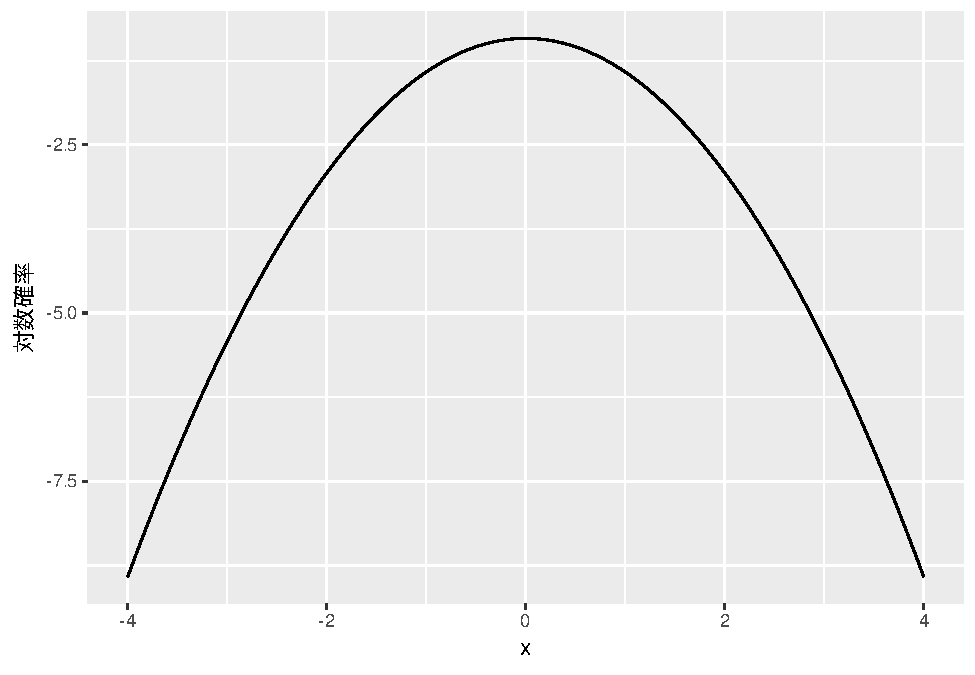
\includegraphics[width=1\linewidth,height=1\textheight,keepaspectratio]{addendum_files/figure-latex/plot-example-1} 

}

\caption{標準正規分布}\label{fig:plot-example}
\end{figure}

先ほどのグラフは, R コードチャンクで描いています. そしてチャンクラベルは \texttt{plot-example} です. このとき, ラベルの頭に \texttt{fig:} を付けたものが図の参照IDになります. よって, \texttt{\textbackslash{}@ref(fig:plot-example)} で図番号を自動で挿入できます (図\ref{fig:plot-example}). 「図: XXXX」のキャプション部分は, チャンクオプション \texttt{fig.cap=} で設定できます.

表も同様ですが, 表のタイトルを付ける場合は \texttt{knitr::kable()} や \texttt{kableExtra::kbl()} が必要になります (表\ref{tab:table-example}). 表を参照する場合, \texttt{\textbackslash{}@ref(tab:table-example)} のように, チャンクラベルに \texttt{tab:} を付ける必要があります.

\begin{Shaded}
\begin{Highlighting}[numbers=left,,]
\FunctionTok{data}\NormalTok{(mtcars)}
\NormalTok{knitr}\SpecialCharTok{::}\FunctionTok{kable}\NormalTok{(}\FunctionTok{head}\NormalTok{(mtcars), }\AttributeTok{caption =} \StringTok{"表の例"}\NormalTok{, }\AttributeTok{booktabs =}\NormalTok{ T)}
\end{Highlighting}
\end{Shaded}

\begin{table}

\caption{\label{tab:table-example}表の例}
\centering
\begin{tabular}{lrrrrrrrrrrr}
\toprule
  & mpg & cyl & disp & hp & drat & wt & qsec & vs & am & gear & carb\\
\midrule
Mazda RX4 & 21.0 & 6 & 160 & 110 & 3.90 & 2.620 & 16.46 & 0 & 1 & 4 & 4\\
Mazda RX4 Wag & 21.0 & 6 & 160 & 110 & 3.90 & 2.875 & 17.02 & 0 & 1 & 4 & 4\\
Datsun 710 & 22.8 & 4 & 108 & 93 & 3.85 & 2.320 & 18.61 & 1 & 1 & 4 & 1\\
Hornet 4 Drive & 21.4 & 6 & 258 & 110 & 3.08 & 3.215 & 19.44 & 1 & 0 & 3 & 1\\
Hornet Sportabout & 18.7 & 8 & 360 & 175 & 3.15 & 3.440 & 17.02 & 0 & 0 & 3 & 2\\
\addlinespace
Valiant & 18.1 & 6 & 225 & 105 & 2.76 & 3.460 & 20.22 & 1 & 0 & 3 & 1\\
\bottomrule
\end{tabular}
\end{table}

\textbf{kableExtra} パッケージがあると, 表を装飾できます (表\ref{tab:table-example2}).

\begin{Shaded}
\begin{Highlighting}[numbers=left,,]
\FunctionTok{require}\NormalTok{(kableExtra)}
\NormalTok{mtcars[}\DecValTok{1}\SpecialCharTok{:}\DecValTok{8}\NormalTok{, }\DecValTok{1}\SpecialCharTok{:}\DecValTok{8}\NormalTok{] }\SpecialCharTok{\%\textgreater{}\%}
  \FunctionTok{kbl}\NormalTok{(}\AttributeTok{caption =} \StringTok{"kableExtra でスタイルを設定した表"}\NormalTok{, }\AttributeTok{booktabs =}\NormalTok{ T) }\SpecialCharTok{\%\textgreater{}\%}
  \FunctionTok{kable\_paper}\NormalTok{(}\AttributeTok{full\_width =}\NormalTok{ F) }\SpecialCharTok{\%\textgreater{}\%}
  \FunctionTok{column\_spec}\NormalTok{(}\DecValTok{2}\NormalTok{,}
    \AttributeTok{color =} \FunctionTok{spec\_color}\NormalTok{(mtcars}\SpecialCharTok{$}\NormalTok{mpg[}\DecValTok{1}\SpecialCharTok{:}\DecValTok{8}\NormalTok{]),}
    \AttributeTok{link =} \StringTok{"https://haozhu233.github.io/kableExtra/"}
\NormalTok{  ) }\SpecialCharTok{\%\textgreater{}\%}
  \FunctionTok{column\_spec}\NormalTok{(}\DecValTok{6}\NormalTok{,}
    \AttributeTok{color =} \StringTok{"white"}\NormalTok{,}
    \AttributeTok{background =} \FunctionTok{spec\_color}\NormalTok{(mtcars}\SpecialCharTok{$}\NormalTok{drat[}\DecValTok{1}\SpecialCharTok{:}\DecValTok{8}\NormalTok{], }\AttributeTok{end =} \FloatTok{0.7}\NormalTok{),}
    \AttributeTok{popover =} \FunctionTok{paste}\NormalTok{(}\StringTok{"am:"}\NormalTok{, mtcars}\SpecialCharTok{$}\NormalTok{am[}\DecValTok{1}\SpecialCharTok{:}\DecValTok{8}\NormalTok{])}
\NormalTok{  )}
\end{Highlighting}
\end{Shaded}

\begin{table}

\caption{\label{tab:table-example2}kableExtra でスタイルを設定した表}
\centering
\begin{tabular}{l>{}rrrr>{}rrrr}
\toprule
  & mpg & cyl & disp & hp & drat & wt & qsec & vs\\
\midrule
Mazda RX4 & \href{https://haozhu233.github.io/kableExtra/}{\textcolor[HTML]{34B679}{21.0}} & 6 & 160.0 & 110 & \cellcolor[HTML]{43BF71}{\textcolor{white}{3.90}} & 2.620 & 16.46 & 0\\
Mazda RX4 Wag & \href{https://haozhu233.github.io/kableExtra/}{\textcolor[HTML]{34B679}{21.0}} & 6 & 160.0 & 110 & \cellcolor[HTML]{43BF71}{\textcolor{white}{3.90}} & 2.875 & 17.02 & 0\\
Datsun 710 & \href{https://haozhu233.github.io/kableExtra/}{\textcolor[HTML]{95D840}{22.8}} & 4 & 108.0 & 93 & \cellcolor[HTML]{37B878}{\textcolor{white}{3.85}} & 2.320 & 18.61 & 1\\
Hornet 4 Drive & \href{https://haozhu233.github.io/kableExtra/}{\textcolor[HTML]{44BF70}{21.4}} & 6 & 258.0 & 110 & \cellcolor[HTML]{414387}{\textcolor{white}{3.08}} & 3.215 & 19.44 & 1\\
Hornet Sportabout & \href{https://haozhu233.github.io/kableExtra/}{\textcolor[HTML]{26818E}{18.7}} & 8 & 360.0 & 175 & \cellcolor[HTML]{3C4F8A}{\textcolor{white}{3.15}} & 3.440 & 17.02 & 0\\
\addlinespace
Valiant & \href{https://haozhu233.github.io/kableExtra/}{\textcolor[HTML]{2C728E}{18.1}} & 6 & 225.0 & 105 & \cellcolor[HTML]{440154}{\textcolor{white}{2.76}} & 3.460 & 20.22 & 1\\
Duster 360 & \href{https://haozhu233.github.io/kableExtra/}{\textcolor[HTML]{440154}{14.3}} & 8 & 360.0 & 245 & \cellcolor[HTML]{375A8C}{\textcolor{white}{3.21}} & 3.570 & 15.84 & 0\\
Merc 240D & \href{https://haozhu233.github.io/kableExtra/}{\textcolor[HTML]{FDE725}{24.4}} & 4 & 146.7 & 62 & \cellcolor[HTML]{1FA187}{\textcolor{white}{3.69}} & 3.190 & 20.00 & 1\\
\bottomrule
\end{tabular}
\end{table}

ただし, 上記は Word の場合はうまく行かないかもしれません. Word に限って言えば \textbf{flextable} パッケージを使ったほうが良い出力を得やすいようです.

詳細は公式のドキュメントを参照してください.

\url{https://cran.r-project.org/web/packages/kableExtra/vignettes/awesome_table_in_html.html}

\hypertarget{ux3088ux308aux8a73ux7d30ux306aux53c2ux8003ux8cc7ux6599-markdown-ux69cbux6587}{%
\subsubsection{より詳細な参考資料: Markdown 構文}\label{ux3088ux308aux8a73ux7d30ux306aux53c2ux8003ux8cc7ux6599-markdown-ux69cbux6587}}

Markdown 構文全般の説明は, Definitive Guide の \href{https://bookdown.org/yihui/rmarkdown/markdown-syntax.html}{2.5}節などが網羅的です. Markdown にはいろいろな方言があるため, R Markdown 以外の Markdown 構文の解説は R Markdown では使えないことがあることに注意してください. 基本的に, R Markdown または Pandoc を想定した Markdown の解説を参照するとよいでしょう.

\hypertarget{YAML}{%
\section{YAML メタデータについてより詳しく}\label{YAML}}

\hypertarget{yaml-ux30e1ux30bfux30c7ux30fcux30bfux306eux57faux672cux69cbux6587}{%
\subsection{YAML メタデータの基本構文}\label{yaml-ux30e1ux30bfux30c7ux30fcux30bfux306eux57faux672cux69cbux6587}}

ここまで, タイトルや \texttt{output} しか設定していなかった YAML メタデータについて詳しく説明します.

Rmd ファイルの冒頭の \texttt{-\/-\/-\/-} で囲まれた範囲は YAML メタデータといいます. この部分の構文は YAML という構文で書かれています. YAML はデータを記述するためのものですが, 例えば JSON と比べると Markdown に似ており視覚的に見やすいという利点があります. 典型的なものは

\begin{Shaded}
\begin{Highlighting}[]
\PreprocessorTok{{-}{-}{-}{-}}
\FunctionTok{title}\KeywordTok{:}\AttributeTok{ }\StringTok{"タイトル"}
\FunctionTok{output}\KeywordTok{:}\AttributeTok{ html\_document}
\PreprocessorTok{{-}{-}{-}{-}}
\end{Highlighting}
\end{Shaded}

のように, 常に \texttt{フィールド名:\ 値} という形で書かれます. さらに, インデントをとることでネストさせることもできます.

\begin{Shaded}
\begin{Highlighting}[]
\FunctionTok{output}\KeywordTok{:}
\AttributeTok{  }\FunctionTok{html\_document}\KeywordTok{:}\AttributeTok{ default}
\AttributeTok{  }\FunctionTok{pdf\_document}\KeywordTok{:}\AttributeTok{ default}
\end{Highlighting}
\end{Shaded}

これは出力フォーマットに \texttt{html\_document} と \texttt{pdf\_document} の2つを指定していることを意味します.

リスト (R のリストではなく, 複数の値を並べたもの, という意味) は2通りの書き方があります. 任意の数の値を与えられるフィールドに対して使います. 例えば著者が複数いる場合, 以下2つは同じです.

\begin{Shaded}
\begin{Highlighting}[]
\FunctionTok{author}\KeywordTok{:}\AttributeTok{ }\KeywordTok{[}\StringTok{"R太郎"}\KeywordTok{,}\AttributeTok{ }\StringTok{"R花子"}\KeywordTok{]}
\FunctionTok{output}\KeywordTok{:}\AttributeTok{ html\_document}
\end{Highlighting}
\end{Shaded}

\begin{Shaded}
\begin{Highlighting}[]
\FunctionTok{author}\KeywordTok{:}
\AttributeTok{  }\KeywordTok{{-}}\AttributeTok{  }\StringTok{"R太郎"}
\AttributeTok{  }\KeywordTok{{-}}\AttributeTok{  }\StringTok{"R花子"}
\FunctionTok{output}\KeywordTok{:}\AttributeTok{ html\_document}
\end{Highlighting}
\end{Shaded}

文書の概要を記入する \texttt{abstruct} フィールドなどは, 長いため1行に収めるのが難しいかもしれません. 以下のように \texttt{\textbar{}} または \texttt{\textgreater{}} を使えば複数行にわたるテキストが1つの値とみなされます.

\begin{Shaded}
\begin{Highlighting}[]
\FunctionTok{abstruct}\KeywordTok{: }\CharTok{|}
\NormalTok{  複数行に分けて書きたい場合は}
\NormalTok{  このようにバー (\textasciigrave{}|\textasciigrave{}) を使います}
\end{Highlighting}
\end{Shaded}

\begin{Shaded}
\begin{Highlighting}[]
\FunctionTok{abstruct}\KeywordTok{: }\CharTok{\textgreater{}}
\NormalTok{  複数行に分けて書きたい場合は}
\NormalTok{  このように不等号 (\textasciigrave{}\textgreater{}\textasciigrave{}) も使えます}
\end{Highlighting}
\end{Shaded}

コロン (\texttt{:}) など構文で使われる特殊な記号を値に含めたい場合は, 値全体を引用符で囲んでください.

ここまでは Rmd に限らない YAML メタデータの一般的なルールです.

技術的な補足: R Markdown の YAML メタデータは Pandoc の仕様を利用しています.

\hypertarget{yaml-ux30e1ux30bfux30c7ux30fcux30bfux3067ux306eux8a2dux5b9a}{%
\subsection{YAML メタデータでの設定}\label{yaml-ux30e1ux30bfux30c7ux30fcux30bfux3067ux306eux8a2dux5b9a}}

R Markdown では YAML メタデータのほとんどにデフォルト値が設定されているため, 一切書かなくても出力できる事が多いです. デフォルトでは \texttt{output:\ html\_document} なので, HTML 形式のレポートが出力されます.

しかしおそらく最低限の設定は必要でしょう. 例えばセッションで使用したように, タイトル・著者・出力フォーマットの設定は最低限必要でしょう.

\begin{Shaded}
\begin{Highlighting}[]
\PreprocessorTok{{-}{-}{-}{-}}
\FunctionTok{title}\KeywordTok{:}\AttributeTok{ }\StringTok{"タイトル"}
\FunctionTok{author}\KeywordTok{:}\AttributeTok{ }\StringTok{"氏名"}
\FunctionTok{output}\KeywordTok{:}\AttributeTok{ bookdown::html\_document2}
\PreprocessorTok{{-}{-}{-}{-}}
\end{Highlighting}
\end{Shaded}

R Markdown の YAML メタデータの設定で一番重要かつ, 初心者にわかりにくいのは \texttt{output} フィールドだと思われます. ここには R Markdown 出力フォーマットを指定します. 出力フォーマットとは, R の関数です. デフォルトでは \texttt{rmarkdown::html\_document} が使用されます. \texttt{html\_document} のように \textbf{rmarkdown} パッケージに含まれている関数は, パッケージ名を書かなくてもよいですが, それ以外は上記のように \texttt{パッケージ名::} が必要になります.

スタイルを調整したい場合の多くは, \texttt{ouput:} 以下にさらに設定をネストして書くことになります. この項目は膨大で, かつフォーマットによって異なります. しかし, 出力フォーマットは R の関数であり, 出力フォーマットにネストできる項目が引数と同じであると分かれば簡単に調べることができます. つまり, (普通は) ヘルプページが用意されています.

\begin{Shaded}
\begin{Highlighting}[]
\PreprocessorTok{{-}{-}{-}{-}}
\FunctionTok{output}\KeywordTok{:}
\AttributeTok{  }\FunctionTok{html\_document}\KeywordTok{:}
\AttributeTok{    }\FunctionTok{code\_folding}\KeywordTok{:}\AttributeTok{ hide}\CommentTok{  \# コードを折りたたんで表示する}
\AttributeTok{    }\FunctionTok{number\_sections}\KeywordTok{:}\AttributeTok{ }\CharTok{yes}\CommentTok{  \# セクション番号を表示する}
\PreprocessorTok{{-}{-}{-}{-}}
\end{Highlighting}
\end{Shaded}

なお, R の \texttt{TRUE}/\texttt{FALSE} に対応する値は, \texttt{true}/\texttt{false}, \texttt{yes}/\texttt{no} で置き換えることができます.

YAML の記入ミスがあった場合のエラーメッセージは少々わかりにくいです.

手動の記入に自信がないなら, \textbf{ymlthis} パッケージをインストールすると, RStudio の アドインから ``Write New R Markdown or YAML File'' を選んで設定用のダイアログボックスを開けます (図\ref{fig:ymlthis}). ただし, 出力フォーマットの項目は \textbf{rmarkdown} で提供されているものにのみ対応しています.



\begin{Shaded}
\begin{Highlighting}[numbers=left,,]
\NormalTok{knitr}\SpecialCharTok{::}\FunctionTok{include\_graphics}\NormalTok{(}\StringTok{"img/ymlthis.png"}\NormalTok{)}
\end{Highlighting}
\end{Shaded}

\begin{figure}

{\centering 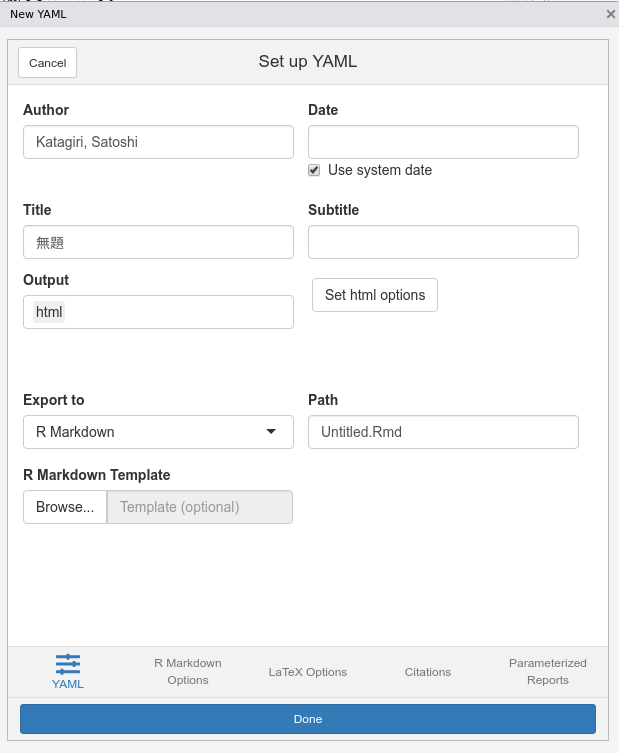
\includegraphics[width=1\linewidth,height=1\textheight,keepaspectratio]{img/ymlthis} 

}

\caption{\textbf{ymlthis} の画面}\label{fig:ymlthis}
\end{figure}

現状, 出力フォーマットで設定できる項目 (\texttt{output:} にネストされている項目) と, YAML メタデータのトップレベルに使用できる項目にはいくつか重複しているものがあり, 注意が必要です.

\hypertarget{ux753bux50cfux306eux51faux529b}{%
\section{画像の出力}\label{ux753bux50cfux306eux51faux529b}}

\hypertarget{ux30b0ux30e9ux30d5ux30a3ux30c3ux30afux30c7ux30d0ux30a4ux30b9}{%
\subsection{グラフィックデバイス}\label{ux30b0ux30e9ux30d5ux30a3ux30c3ux30afux30c7ux30d0ux30a4ux30b9}}

すでに R に慣れている人はご存知と思いますが, R のグラフィックに日本語のタイトルやラベルを含む場合, 環境によっては文字化けします. そしてその解決法が OS によって異なるため, 情報の錯綜と混乱を生んできました\footnote{この問題は \url{https://ill-identified.hatenablog.com/entry/2020/10/03/200618} に詳しく書きましたが, 今は読まなくても大丈夫です.}.

しかし, 最近登場した \textbf{ragg} パッケージ v1.1.0 により, この問題は劇的に改善されました.

\begin{enumerate}
\def\labelenumi{\arabic{enumi}.}
\tightlist
\item
  Windows ではデフォルトの \texttt{png} デバイスより描画が美しい
\item
  主要な OS で, 特に指定がなくとも日本語フォントにフォールバックされる
\end{enumerate}

という利点があります. よって文字化け問題に対して無用の労力をかける必要がなくなりました. 今回の資料でも最初にインストールすることをお薦めしています.

R Markdown では多くの場合グラフィックデバイスのデフォルトが \texttt{png} なので, 今回は明示的に \texttt{ragg\_png} に指定しています. 一方で, ベクタ画像が良いという場合は \textbf{svglite} パッケージによる \texttt{svglite} を指定することができます.

ただしこれは HTML/Word 出力の場合です. PDF の場合, 画像も PDF 形式にできます. PDF ではフォントの変更はよりシビアなため, \texttt{pdf} ではなくより使いやすい \texttt{cairo\_pdf} の指定をおすすめします. X11 や cairo を確認させたのはこれが理由です.

\hypertarget{ux30b5ux30a4ux30baux306eux8abfux6574}{%
\subsection{サイズの調整}\label{ux30b5ux30a4ux30baux306eux8abfux6574}}

R Markdown では画像サイズを決めるのに大きく分けて2種類のパラメータがあります. Markdown 記法は既存の画像ファイルを貼り付けるものでしたが, コードチャンクでは, 内部でグラフを生成し, 画像として保存, そして文書に貼り付ける, という動作をしています. よって, 保存時のサイズと文書掲載時のサイズをそれぞれ決めるパラメータが存在します.

\begin{itemize}
\item
  \texttt{fig.width}, \texttt{fig.height} などは保存時のサイズで, \textbf{単位はインチ}です.
\item
  \texttt{out.height}, \texttt{out.width} などは掲載時のサイズで, \textbf{単位は出力フォーマットに依存します}.
\end{itemize}

しかし基本的には余白に対するパーセント表記で決めると簡単でしょう.

これの使いにくいところは, 例えばグラフ内の文字が出力時にどれくらいの大きさになるかがわかりにくい点です. 自分でなにかルールを決めたり, オプションフックで自動調整する関数を書くという手があります\footnote{オプションフックは Yihui 氏の解説が参考になります. 翻訳したものをご覧ください \url{https://gedevan-aleksizde.github.io/knitr-doc-ja/hooks.html\#\%E3\%82\%AA\%E3\%83\%97\%E3\%82\%B7\%E3\%83\%A7\%E3\%83\%B3\%E3\%83\%95\%E3\%83\%83\%E3\%82\%AF}}.

\hypertarget{pdf-intro}{%
\section{PDF 出力の内幕}\label{pdf-intro}}

R Markdown で PDF を出力する場合, \texttt{.md} ファイルを pandoc で \texttt{.tex} 形式に変換してから LaTeX で PDF を生成します (この作業をコンパイルといいます). このとき, LaTeX プログラムの呼び出しを \textbf{tinytex} パッケージで制御しています.

まだ LaTeX をインストールして使用したことがない場合は, \textbf{tinytex} で簡単にインストールすることもできます. これはチュートリアルの環境設定にも書かれている, 以下のコマンドで実行できます. 2行目は必ずしも必要ではありませんが, 日本語ロケールだと毎回警告が出て邪魔なのでインストールしましょう.

\begin{Shaded}
\begin{Highlighting}[numbers=left,,]
\NormalTok{tinytex}\SpecialCharTok{::}\FunctionTok{install\_tinytex}\NormalTok{()}
\NormalTok{tinytex}\SpecialCharTok{::}\FunctionTok{tlmgr\_install}\NormalTok{(}\StringTok{"texlive{-}msg{-}translations"}\NormalTok{)}
\end{Highlighting}
\end{Shaded}

ただしこれは\textbf{必須ではありません}. 既に LaTeX をインストールしていると\textbf{競合します}. 注意してください.

LaTeX で PDF をコンパイルする場合, 様々なプログラムを複数回呼び出す必要があります. それを制御するのが \textbf{tinytex} の役目の1つです. この役目は従来 latexmk というプログラムが担っていましたが, \textbf{tinytex} は latexmk の処理をエミュレートすることができます. その結果, エラー発生箇所の追跡が多少簡単になりました.

詳細は R Markdown クックブックの \href{https://gedevan-aleksizde.github.io/rmarkdown-cookbook/install-latex.html}{1.2}, \href{https://gedevan-aleksizde.github.io/rmarkdown-cookbook/install-latex-pkgs.html}{1.3}節を見てください

latexmk エミュレーションを無効にする必要のある場面として, 後述する (u)pBibTeX を使用するというものがあります.

latexmk の使用法は以下が参考になります (必須ではありません).

\begin{itemize}
\tightlist
\item
  \url{https://texwiki.texjp.org/?Latexmk}
\item
  \url{http://www2.yukawa.kyoto-u.ac.jp/~koudai.sugimoto/dokuwiki/doku.php?id=latex:latexmk\%E3\%81\%AE\%E8\%A8\%AD\%E5\%AE\%9A}
\end{itemize}

\hypertarget{latex-ux306eux51faux529bux30a8ux30f3ux30b8ux30f3}{%
\subsection{LaTeX の出力エンジン}\label{latex-ux306eux51faux529bux30a8ux30f3ux30b8ux30f3}}

R Markdown が使用できる LaTeX エンジンは基本的に以下の3つです.

\begin{enumerate}
\def\labelenumi{\arabic{enumi}.}
\tightlist
\item
  \texttt{pdflatex} (pdfLaTeX)
\item
  \texttt{xelatex} (XeLaTeX)
\item
  \texttt{lualatex} (LuaLaTeX\footnote{実際には LuaHBTeX})
\item
  \texttt{tectonic}\footnote{\textbf{rmarkdown} \textgreater= 2.8 でサポート予定}
\end{enumerate}

つまり, 基本エンジンである LaTeX2e ひいては pLaTeX (pLaTeX2e) での使用は実は想定されていません\footnote{英語圏の開発者は必ずしも日本語 LaTeX 事情を把握していないためです: \url{https://acetaminophen.hatenablog.com/entry/texadvent2020}}. (1) は欧文での処理のスタンダードになっています. これで日本語文書をコンパイルする場合, 不可能ではありませんが難しい and 使用例が少ないため候補から外れます. 最近は日本語文書を (2, 3) でコンパイルする例が増えています. (4) は最近登場し, Pandoc もサポートするようになったため, 次にリリースされるバージョンからサポートされます. ただし, XeTeX ベースなので出力は基本的に \texttt{xelatex} と変わらないはずです. また, BibTeX/BibLaTeX, MakeIndex 等への対応も不十分なようです. よって通常は, (2, 3) のどちらかを使うことをおすすめします.

(2, 3) についてはそれぞれ特性が異なります. \texttt{xelatex} はよりコンパイルが速いですが, 和文の禁則処理の一部が甘いです. 逆に \texttt{lualatex} はより利用が活発なためか禁則処理がより厳格ですが, 一方でより処理速度が遅くなっています. それ以外にも対応している文書クラスの設定が微妙に異なるなどの違いがあります. 個人的な体感として, 短い文書であれば速度はあまり気になりません. また, スライドであれば \texttt{xelatex} の禁則処理の甘さも気になる場面が減ると思います. これも個人的な考えですが, 普段は \texttt{xelatex} を使い, 完成版は時間のかかる \texttt{lualatex} に切り替える, ということをしています\footnote{TeX Live 開発に関わっている日本人はなるべく LuaLaTeX を使うように主張しています.}. ただし, 両者の互換性をよく理解していないとこのやり方はうまくいかないこともあります.

\hypertarget{r-markdown-ux3068-latex-ux30c6ux30f3ux30d7ux30ecux30fcux30c8ux306eux878dux5408}{%
\subsection{R Markdown と LaTeX テンプレートの融合}\label{r-markdown-ux3068-latex-ux30c6ux30f3ux30d7ux30ecux30fcux30c8ux306eux878dux5408}}

あなたが独自にカスタマイズした LaTeX のテンプレートを組み込んで, R Markdown で使用できれば便利でしょう.

LaTeX のテンプレートを R Markdown から操作する3つの主な方法があります.

\begin{enumerate}
\def\labelenumi{\arabic{enumi}.}
\tightlist
\item
  YAML メタデータの設定項目 (Pandoc の機能)
\item
  Pandoc テンプレートの改造
\item
  プリアンブルに部分的に挿入する
\end{enumerate}

まず, (1) は \texttt{documentclass} および \texttt{classoption} です. それぞれ, \texttt{.tex} ファイル冒頭の \texttt{\textbackslash{}documentclass{[}{]}\{\}} の文書クラスとオプションに代入されます. article, report, book といったカスタマイズは, このオプションだけで十分でしょう.

R Markdown は, knit で処理した本文と YAML メタデータを Pandoc のテンプレートに代入します. ターミナルで
\texttt{bash\ \ \ \ \ pandoc\ -D\ latex\ \textgreater{}\ latex.template.tex}
を実行してみてください. Pandoc の LaTeX 用テンプレートファイルが出力されます. これはほぼ \texttt{.tex} ファイルですが, 至るところに \texttt{\$documentclass\$} のような Pandoc マクロが含まれています. これは主に (1) の YAML メタデータで入力した項目が代入されます. このマクロに注意しつつあなたのテンプレートを移植することができます. デフォルトのテンプレートは日本語出力が十分に考慮されていないことの改善や, より視覚的に優れたデザインにするため, \textbf{rmdja} はデフォルトのものを改造した独自の LaTeX テンプレートを使用しています. 詳細は『R Markdown Cookbook』\href{https://gedevan-aleksizde.github.io/rmarkdown-cookbook/latex-variables.html}{6.2}, \href{https://gedevan-aleksizde.github.io/rmarkdown-cookbook/latex-template.html}{6.10}節や Pandoc の公式ドキュメント\footnote{ \url{https://pandoc.org/MANUAL.html\#variables-for-latex}} を参考にしてください.

マクロも自分で新規に定義できます. \textbf{rmdja} ではフォントの選択に自由と利便性をもたせるため, \texttt{jamainfont}, \texttt{jasansfont}, \texttt{jamonofont}, \texttt{jafontpriset} という YAML メタデータのフィールドを新たに定義しています.

特定のパッケージを追加で読み込むとか, 修正箇所がごくわずかなら, (3) の方法が簡単でしょう. 例えば, \textbf{kableExtra} パッケージの機能を beamer で完全に使うには, 追加のパッケージが必要と公式ドキュメント\footnote{\url{https://haozhu233.github.io/kableExtra/}}に書かれています\footnote{\textbf{rmdja} の beamer フォーマットでは, これらのパッケージの読み込みコマンドを内蔵済みです.}. それは YAML メタデータに以下のように追記して実現できます.

\begin{Shaded}
\begin{Highlighting}[]
\FunctionTok{header{-}includes}\KeywordTok{:}
\AttributeTok{  }\KeywordTok{{-}}\AttributeTok{ \textbackslash{}usepackage\{booktabs\}}
\AttributeTok{  }\KeywordTok{{-}}\AttributeTok{ \textbackslash{}usepackage\{longtable\}}
\AttributeTok{  }\KeywordTok{{-}}\AttributeTok{ \textbackslash{}usepackage\{array\}}
\AttributeTok{  }\KeywordTok{{-}}\AttributeTok{ \textbackslash{}usepackage\{multirow\}}
\AttributeTok{  }\KeywordTok{{-}}\AttributeTok{ \textbackslash{}usepackage\{wrapfig\}}
\AttributeTok{  }\KeywordTok{{-}}\AttributeTok{ \textbackslash{}usepackage\{float\}}
\AttributeTok{  }\KeywordTok{{-}}\AttributeTok{ \textbackslash{}usepackage\{colortbl\}}
\AttributeTok{  }\KeywordTok{{-}}\AttributeTok{ \textbackslash{}usepackage\{pdflscape\}}
\AttributeTok{  }\KeywordTok{{-}}\AttributeTok{ \textbackslash{}usepackage\{tabu\}}
\AttributeTok{  }\KeywordTok{{-}}\AttributeTok{ \textbackslash{}usepackage\{threeparttable\}}
\AttributeTok{  }\KeywordTok{{-}}\AttributeTok{ \textbackslash{}usepackage\{threeparttablex\}}
\AttributeTok{  }\KeywordTok{{-}}\AttributeTok{ \textbackslash{}usepackage[normalem]\{ulem\}}
\AttributeTok{  }\KeywordTok{{-}}\AttributeTok{ \textbackslash{}usepackage\{makecell\}}
\AttributeTok{  }\KeywordTok{{-}}\AttributeTok{ \textbackslash{}usepackage\{xcolor\}}
\end{Highlighting}
\end{Shaded}

ただし, パッケージのロードの順番によってエラーが起きることもあるので注意してください. 例えば色を変えたりグラフィックをいじったりするタイプのパッケージは追加を要求される可能性が高い上に競合しやすいです.

なお, LaTeXパッケージを読み込むだけならば, 出力フォーマットの引数 \texttt{extra\_dependencies} が使えることもあります (『R Markdown クックブック』6.4節).

\begin{Shaded}
\begin{Highlighting}[]
\FunctionTok{output}\KeywordTok{:}
\AttributeTok{  }\FunctionTok{pdf\_document}\KeywordTok{:}
\AttributeTok{    }\FunctionTok{extra\_dependencies}\KeywordTok{:}
\AttributeTok{      }\KeywordTok{{-}}\AttributeTok{ booktabs}
\AttributeTok{      }\KeywordTok{{-}}\AttributeTok{ longtable}
\AttributeTok{      ...}
\AttributeTok{      }\KeywordTok{{-}}\AttributeTok{ xcolor}
\end{Highlighting}
\end{Shaded}

別の方法として, PDF 系の出力フォーマットの多くには \texttt{includes} 引数があります.

\begin{Shaded}
\begin{Highlighting}[]
\FunctionTok{output}\KeywordTok{:}
\AttributeTok{  }\FunctionTok{pdf\_document}\KeywordTok{:}
\AttributeTok{    }\FunctionTok{includes}\KeywordTok{:}
\AttributeTok{      }\FunctionTok{in\_header}\KeywordTok{:}\AttributeTok{ preamble.tex}
\AttributeTok{      }\FunctionTok{before\_body}\KeywordTok{:}\AttributeTok{ before{-}body.tex}
\AttributeTok{      }\FunctionTok{after\_body}\KeywordTok{:}\AttributeTok{ after{-}body.tex}
\end{Highlighting}
\end{Shaded}

カスタマイズの多くはプリアンブルでなされるので, 設定を記入したファイルを別に作り, \texttt{in\_header:\ preamble.tex} のように指定します. \texttt{before} は \texttt{document} 環境, つまり本文開始直後に挿入されます. よって洋書によくある冒頭のエピグラフや「誰々に捧げる」的な文章や, あるいはロゴマークを挿入するのに使えます. \texttt{after\_body} も本文の最後に挿入されます. PDF版にのみ巻末索引や付録を付ける場合に使いますが, これらは他の方法でも代替可能 (cf.~\texttt{knitr::is\_latex\_output()} で条件出力させる) であることが多いのであまり使わないかもしれません.

\texttt{include-headers} と \texttt{includes} の違いは, 前者はトップレベルの YAML メタデータなので PDF 以外のフォーマットにも入力されるということです. ほとんどの場合は無害ですが, もし HTML と PDF で異なる入力が必要な場合, \texttt{includes} を使うことになるでしょう. また, LaTeX とそれ以外のソースを別ファイルに分けることは保守性の改善につながるかもしれません.

\begin{infobox}{important}
フォーマットによっては, \texttt{in\_header} が \texttt{header-includes} を上書きしてしまうことがあるので注意してください.

\end{infobox}

ただし, (u)pLaTeX など R Markdown が対応していない LaTeX エンジンに依存したテンプレートの場合, これだけでは「knit ボタンで一発コンパイル」ということはできません, 残念ながら. それは次のセクションを参考にしてください.

\hypertarget{ux30b5ux30ddux30fcux30c8ux5916ux306e-latex-ux30a8ux30f3ux30b8ux30f3ux3092ux4f7fux7528ux3059ux308b}{%
\subsection{サポート外の LaTeX エンジンを使用する}\label{ux30b5ux30ddux30fcux30c8ux5916ux306e-latex-ux30a8ux30f3ux30b8ux30f3ux3092ux4f7fux7528ux3059ux308b}}

昔からある (u)pLaTeX などでのコンパイルを前提としたテンプレートを使う必要のある場面も多いと思います. これらを使うもっとも確実な方法は, .tex ファイルを出力して, 手動でコンパイルすることです. 現時点では, (u)pLaTeX で使えない設定が書かれていることが多いので, 手動で書き換えることも必要になります.

現時点では, \texttt{rmja::beamer\_presentation\_jp} は XeLaTeX と LuaLaTeX のみの使用を前提としており, それ以外のサポートの予定はありません. プレゼン資料については体裁の厳格な制約がないものと考えているからです.

\hypertarget{biblio}{%
\section{参考文献スタイルのカスタマイズ}\label{biblio}}

\hypertarget{ux53c2ux8003ux6587ux732eux8a2dux5b9aux306eux57faux672cux4e8bux9805}{%
\subsection{参考文献設定の基本事項}\label{ux53c2ux8003ux6587ux732eux8a2dux5b9aux306eux57faux672cux4e8bux9805}}

参考文献リストの出力方法は以下の4通りの方法があります.

\begin{enumerate}
\def\labelenumi{\arabic{enumi}.}
\tightlist
\item
  \texttt{default} (CSL)
\item
  \texttt{natbib} (BibTeX)
\item
  \texttt{biblatex} (BibLaTeX)
\item
  手動で書き込む
\end{enumerate}

~(4) は文字通りなので省略します. (1 - 3) は文献データベースに登録したものを, 本文の引用されたものだけを自動的に取り出して一覧を出力します.

~(1) は HTML, PDF, Word いずれにも使えます. (2, 3) は PDF のみです.

共通箇所は YAML で, 出力スタイルの設定と, \texttt{bibliography} フィールドで文献データベースファイルを指定することです.

\begin{Shaded}
\begin{Highlighting}[]
\FunctionTok{output}\KeywordTok{:}
\AttributeTok{    }\FunctionTok{XXX\_output}\KeywordTok{:}
\AttributeTok{      }\FunctionTok{citation\_package}\KeywordTok{:}\AttributeTok{ ENGINE}
\FunctionTok{bibliography}\KeywordTok{:}\AttributeTok{ REFS.bib}
\end{Highlighting}
\end{Shaded}

\texttt{ENGINE} には上記の3つのどれかを指定します. \texttt{REFS.bib} は文献データベースファイルです. 対応可能なファイル形式は RStudio の公式ページの一覧を確認してください.

\url{https://rmarkdown.rstudio.com/authoring_bibliographies_and_citations.html}

また, \texttt{default} の場合に限り, YAML メタデータ内に文献情報を書けるインライン参考文献リスト (inline references) の構文が使用できます. 例えばこのように書きます.

\begin{Shaded}
\begin{Highlighting}[]
\FunctionTok{references}\KeywordTok{:}
\AttributeTok{  }\KeywordTok{{-}}\AttributeTok{ }\FunctionTok{type}\KeywordTok{:}\AttributeTok{ article{-}journal}
\AttributeTok{    }\FunctionTok{id}\KeywordTok{:}\AttributeTok{ WatsonCrick1953}
\AttributeTok{    }\FunctionTok{author}\KeywordTok{:}
\AttributeTok{    }\KeywordTok{{-}}\AttributeTok{ }\FunctionTok{family}\KeywordTok{:}\AttributeTok{ Watson}
\AttributeTok{      }\FunctionTok{given}\KeywordTok{:}\AttributeTok{ J. D.}
\AttributeTok{    }\KeywordTok{{-}}\AttributeTok{ }\FunctionTok{family}\KeywordTok{:}\AttributeTok{ Crick}
\AttributeTok{      }\FunctionTok{given}\KeywordTok{:}\AttributeTok{ F. H. C.}
\AttributeTok{    }\FunctionTok{issued}\KeywordTok{:}
\AttributeTok{      }\FunctionTok{date{-}parts}\KeywordTok{:}
\AttributeTok{      }\KeywordTok{{-}}\AttributeTok{ }\KeywordTok{{-}}\AttributeTok{ }\DecValTok{1953}
\AttributeTok{        }\KeywordTok{{-}}\AttributeTok{ }\DecValTok{4}
\AttributeTok{        }\KeywordTok{{-}}\AttributeTok{ }\DecValTok{25}
\AttributeTok{    }\FunctionTok{title}\KeywordTok{:}\AttributeTok{ }\StringTok{\textquotesingle{}Molecular structure of nucleic acids: a structure for}
\StringTok{      deoxyribose nucleic acid\textquotesingle{}}
\AttributeTok{    }\FunctionTok{title{-}short}\KeywordTok{:}\AttributeTok{ Molecular structure of nucleic acids}
\AttributeTok{    }\FunctionTok{container{-}title}\KeywordTok{:}\AttributeTok{ Nature}
\AttributeTok{    }\FunctionTok{volume}\KeywordTok{:}\AttributeTok{ }\DecValTok{171}
\AttributeTok{    }\FunctionTok{issue}\KeywordTok{:}\AttributeTok{ }\DecValTok{4356}
\AttributeTok{    }\FunctionTok{page}\KeywordTok{:}\AttributeTok{ 737{-}738}
\AttributeTok{    }\FunctionTok{DOI}\KeywordTok{:}\AttributeTok{ 10.1038/171737a0}
\AttributeTok{    }\FunctionTok{URL}\KeywordTok{:}\AttributeTok{ https://www.nature.com/articles/171737a0}
\AttributeTok{    }\FunctionTok{language}\KeywordTok{:}\AttributeTok{ en{-}GB}
\end{Highlighting}
\end{Shaded}

しかし, 基本的には \texttt{.bib} 形式で書いたほうが使いまわしやすいため, \textbf{\texttt{.bib} 形式のファイルを使うことを推奨します}. よって, 以降の解説も \texttt{.bib} ファイルがあるという前提になっています.

特に PDF の出力で, BibTex/BibLaTeX を使用する場合 \texttt{.bib} 形式の文献データベースファイルしか読み込むことができません. これまで LaTeX を使ったことがない, 従って BibTeX も BibLaTeX も使ったことがない, という方は, まずはお持ちの文献リストを \texttt{.bib} ファイルに変換する方法を調べて下さい.

Zotero や Mendeley といった文献管理ソフトの多くには, \texttt{.bib} ファイルをエクスポートする機能があります (前者は better bbx というプラグインも必要です\footnote{Zotero の設定については以下を参考にしてください. \url{https://ill-identified.hatenablog.com/entry/2019/03/05/195257}}) また, CiNii や Google Scholar, あるいは国際学会・学会誌のレポジトリの多くには論文の書誌情報を \texttt{.bib} 形式でエクスポートする機能があるはずです.

文献引用の練習がしたい場合, \texttt{knitr::write\_bib(x\ =\ c("パッケージ名"))} が便利です. これはパッケージ情報を \texttt{.bib} 形式で出力します.

文献データベースが設定できればあとは文中で引用するだけです. \texttt{@文献ID} (\citet{R-rmarkdown}), または \texttt{{[}@文献ID{]}} (\citep{R-bookdown}), \texttt{{[}-@文献)ID{]}} (\citeyearpar{R-citr}) という Markdown 構文が使えます. さらに, セミコロン (\texttt{;}) で区切って複数文献IDを同時に指定できます. 一部の分野では引用が上付き文字\^{}aのようになっているところもあると思います. そのようなケースは CSL 等文献スタイルファイルで制御すると想定されています. PDF 限定でなら, LaTeX コマンドも使えます.

文献IDをいちいち覚えるのが嫌だという方は, \textbf{citr} パッケージによる RStudio アドインが便利です ``Insert Citation'' を押してください\footnote{ただし, bib ファイルの更新を手動で行う必要や, bookdown のように文書を分割しているとうまく動作しなかったり, ややクセがあります.}. Visual Markdown Editor でも ``@ citation'' というボタンを押すとリストが表示されます. こちらは Zotero 等の外部ソフトウェアとの連携や, DOI, PubMed ID などで文献検索もできます (図\ref{fig:vme-citation}).

\begin{Shaded}
\begin{Highlighting}[numbers=left,,]
\NormalTok{knitr}\SpecialCharTok{::}\FunctionTok{include\_graphics}\NormalTok{(}\StringTok{"img/visual{-}editor{-}citation.png"}\NormalTok{)}
\end{Highlighting}
\end{Shaded}

\begin{figure}

{\centering 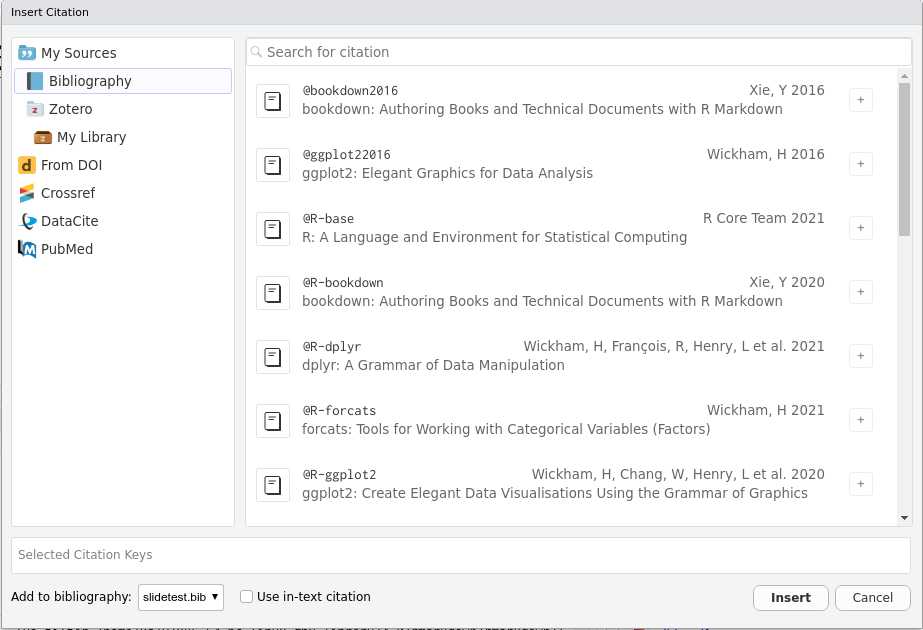
\includegraphics[width=1\linewidth,height=1\textheight,keepaspectratio]{img/visual-editor-citation} 

}

\caption{Visual Markdown Editor による引用リスト}\label{fig:vme-citation}
\end{figure}

参考文献リストのスタイルに拘らないのなら, 設定は以上で十分です. 以降の記述は, おそらくは体裁のルールが細かく決まっている, 例えば,

\begin{itemize}
\tightlist
\item
  {[}1{]} (著者名) ``タイトル (ここは\_イタリック体で\_),'' (出版年), (雑誌名), \ldots{}
\item
  (著者名) (出版年) 『タイトル (ここは太字で)』, (雑誌名), (巻数), \ldots{}
\end{itemize}

といったふうに細かく決まっている学会・ジャーナルを想定した解説になります. 国内の場合, おそらくこれに加えて和・欧文献で引用スタイルが個別に決められていることが多いと思いますので, そのことを念頭に置いた解説をします.

また, 欧文であれば, \href{https://github.com/rstudio/rticles}{\textbf{rticles}} パッケージに既にご専門の分野のテンプレートが作られていないかも確認するとよいでしょう.

引用全般について『R Markdown クックブック』の\href{https://gedevan-aleksizde.github.io/rmarkdown-cookbook/bibliography.html}{4.5}節が参考になります.

\hypertarget{default-csl}{%
\subsection{\texorpdfstring{\texttt{default} (CSL)}{default (CSL)}}\label{default-csl}}

CSL は Microsoft Word でも利用されている文献スタイルフォーマットです. よって, すでに Word をお使いの場合はこのスタイルを使い回すことができます. 特にスタイルにこだわりがないのなら, CSL が最も簡単です. スタイルを指定する場合, 以下のように CSL 形式で記述されたファイルを指定する必要があります.

\begin{Shaded}
\begin{Highlighting}[]
\FunctionTok{output}\KeywordTok{:}
\AttributeTok{    }\FunctionTok{XXX\_output}\KeywordTok{:}
\AttributeTok{      }\FunctionTok{citation\_package}\KeywordTok{:}\AttributeTok{ default}
\FunctionTok{bibliography}\KeywordTok{:}\AttributeTok{ REFS.bib}
\FunctionTok{csl}\KeywordTok{:}\AttributeTok{ my{-}style.csl}
\end{Highlighting}
\end{Shaded}

この \texttt{my-style.csl} に対応するファイルは, 自分で用意する必要があります. 例えば \url{https://www.zotero.org/styles} に IEEE や APA など欧文向けの様々なファイルが配布されています.

\hypertarget{csl-ux306eux30abux30b9ux30bfux30deux30a4ux30baux306bux3064ux3044ux3066}{%
\subsubsection{CSL のカスタマイズについて}\label{csl-ux306eux30abux30b9ux30bfux30deux30a4ux30baux306bux3064ux3044ux3066}}

CSL そのものは XML の構文で書かれおり, \href{https://editor.citationstyles.org/}{CSL Editor} のようなエディタで作ることができ, Zotero によって共有することもできます.

CSL はローカライズには対応していますが, それはスタイル全体で同じ言語を使うことが前提です. 多言語対応に関する開発者らの公式見解としては「文献単位のローカライズは未対応\footnote{``CSL doesn't yet allow for per-item localization,'' \url{https://citationstyles.org/authors/} さらに具体例として日本語ではよくそのようなスタイルを要求されることが名指しで挙げられています.}」とのことです. CSL 開発者らは, この問題に対する代替案として Juris-M の使用を提案しています.

(英語ですが, 該当パートのみすでに第三者により日本語訳されています)

\url{https://juris-m.readthedocs.io/en/latest/tutorial-ja.html}

ただし, Zotero の CSL リポジトリで ``japanese'' と検索すると, いくつかスタイルファイルがヒットします

\url{https://www.zotero.org/styles?q=japanese}

少し技術的な話: PDF の場合は, pandoc-citeproc という Pandoc フィルタを使って, 文献情報を直接書き出します.

\hypertarget{biblatex-biblatex}{%
\subsection{\texorpdfstring{\texttt{biblatex} (BibLaTeX)}{biblatex (BibLaTeX)}}\label{biblatex-biblatex}}

BibLaTeX は PDF 出力の場合のみ有効ですが, LaTeX マクロを使用できるため, CSL に比べてより複雑な組版処理ができます. 典型的な YAML の記述は以下のようになります.

\begin{Shaded}
\begin{Highlighting}[]
\FunctionTok{output}\KeywordTok{:}
\AttributeTok{    }\FunctionTok{XXX\_output}\KeywordTok{:}
\AttributeTok{      }\FunctionTok{citation\_package}\KeywordTok{:}\AttributeTok{ biblatex}
\FunctionTok{bibliography}\KeywordTok{:}\AttributeTok{ REFS.bib}
\FunctionTok{biblio{-}style}\KeywordTok{:}\AttributeTok{ ieee}
\FunctionTok{biblatexoptions}\KeywordTok{:}\AttributeTok{ bibstyle=jauthoryear,citestyle=numeric,natbib=true}
\end{Highlighting}
\end{Shaded}

なお, HTML の場合のために \texttt{csl} フィールドも同時に書くことができます.

新たに登場した2つのフィールドはいずれも任意であり, 必須ではありません. \texttt{biblio-style} は文献リストの体裁を決めるスタイルファイルを指定するフィールドです. デフォルトでは \texttt{numeric} か \texttt{authoryear} が使われます. \texttt{biblatexoptions} はスタイルに関するオプションです. 例えば 上記の例では, 文献リストのスタイル (\texttt{bibstyle}) と引用のスタイル (\texttt{citestyle}) をそれぞれ別のものに設定し, かつ \texttt{natbib.sty} の構文を使えるようにしています (\texttt{natbib.sty} については BibTeX の項目参照). この場合, \texttt{biblio-style} の設定は文献・引用の両方のスタイルを一括して指定していますが, \texttt{bibstyle}, \texttt{citestyle} の設定によってそれぞれ上書きされています. その他にも多くのオプションが存在します. 詳細は BibLaTeX のドキュメント等を確認してください.

BibLaTeX は後述の BibTeX の後継プログラムです. 体裁の設定が LaTeX マクロで定義されているため, (多少) 設定が簡単になりました. BibLaTeX か BibTeX かでいうと, 基本的にはこちらを使ったほうが便利ですが, \textbf{日本語向けのテンプレートはまだ充実していない}というのが現状です.

BiBLaTeX の機能としては, オプション指定のみでいろいろなテンプレートに切り替えられますが, それらは言語別の設定を考慮していません. 特に姓名の順序は日本語とそれ以外で逆転して書くことが多いですが, これも想定されていません. そこで, \textbf{rmdja} パッケージでは\textbf{デフォルトで和欧を分けたスタイルテンプレート, \texttt{jauthoryear.bbx} をロードして使用するようにしました}. デフォルトでスタイルを指定しない場合, 自動でこのスタイルファイルがコピーされ, knit 時に使用されます. このファイルをそのまま使ったり, これを元に必要な体裁に改造したりしてください.

欧文限定ならば, BibLaTeX の主要フォーマットは Overleaf にサンプルが掲載されています.

\url{https://ja.overleaf.com/learn/latex/Biblatex_bibliography_styles}

文献データベースは \texttt{.bib} とほぼ同じものが使えますが, \texttt{jauthoryear} で適切に表示するには以下の2つのフィールドへの記入が必要です.

\begin{enumerate}
\def\labelenumi{\alph{enumi}.}
\tightlist
\item
  \texttt{language} フィールド
\item
  \texttt{yomi} または \texttt{sortname} フィールド
\end{enumerate}

~(a) は和・欧の分類のために必要で, それぞれ \texttt{Japanese}, \texttt{Engilish} と入力してください (他の言語でもたぶん大丈夫です. 保証はしませんが). 例えば BibTeX の \texttt{jecon.bst} は文字コードから言語を判別していましたが, 現時点では \texttt{jauthoryear} にそのような機能はありません.

~(b) は従来の BIbTeX の \texttt{yomi} と同様に, 五十音順を決定するための読みがなを記入するフィールドです. BIbLaTeX では一般には読みによる掲載順は \texttt{sortname} フィールドで指定しますが, \texttt{jauthoryear} では日本語圏での BibTeX との互換性を考え \texttt{yomi} フィールドでも代替できるようにしています. もちろん五十音順でなくてもよいのなら記入しなくてもかまいません. 例えば Zotero ではその他欄に \texttt{tex.yomi:\ ...} と記入することでエクスポートにも反映されます

詳細は私の以前書いたブログ記事を参考にしてください.

\url{https://ill-identified.hatenablog.com/entry/2020/09/20/231335}

\hypertarget{natbib-bibtex}{%
\subsection{\texorpdfstring{\texttt{natbib} (BibTeX)}{natbib (BibTeX)}}\label{natbib-bibtex}}

BibTeX も PDF でのみ有効です. R Markdown では \texttt{natbib} という名称になっています. これは \texttt{natbib.sty} という LaTeX パッケージを使用しているからです. \texttt{natbib.sty} は \texttt{{[}1{]}} のような番号形式や, \texttt{著者\ (年)} 形式などいろいろな表示形式をサポートしています. R Markdown では基本的に \texttt{natbib} と BibTeX がセットになっています. 典型例としては以下のような YAML メタデータを書くことになります.

\begin{Shaded}
\begin{Highlighting}[]
\FunctionTok{output}\KeywordTok{:}
\AttributeTok{  }\FunctionTok{XXX\_document}\KeywordTok{:}
\AttributeTok{    }\FunctionTok{citation\_package}\KeywordTok{:}\AttributeTok{ natbib}
\FunctionTok{bibliography}\KeywordTok{:}\AttributeTok{ REFS.bib}
\FunctionTok{biblio{-}style}\KeywordTok{:}\AttributeTok{ ieee}
\end{Highlighting}
\end{Shaded}

BibLaTeX 同様に, HTML の場合のために \texttt{csl} フィールドも同時に書くことができます.

\texttt{natbib.sty} は, 例えば \texttt{\textbackslash{}citet\{引用ID\}} でテキスト形式引用, \texttt{\textbackslash{}citep\{引用ID\}} で括弧で囲んだ引用, \texttt{\textbackslash{}citeyear\{引用ID\}} で発表年のみ, あるいは \texttt{prettyref.sty} や \texttt{refstyle.sty} と併用することで \texttt{図XX} のように書式付きの引用を行うことができます.\footnote{例えば Overleaf のページ \url{https://www.overleaf.com/learn/latex/natbib_citation_styles} に解説があります. 日本語ですとこのページに出力例があります. \url{http://otoguro.net/home/latex/bibtex/}} ただしこれらは LaTeX コマンドであるため, HTML では反映されません. PDF と HTML で出力を両立させたいなら, Markdown 構文の \texttt{@引用ID}, \texttt{{[}@引用ID{]}} を使用してください.\footnote{実際にはこれら2つは PDF 出力時に Pandoc によって内部でそれぞれ \texttt{\textbackslash{}cite}, \texttt{\textbackslash{}citep} へと変換されています.}

BibTeX の場合, 引用スタイルを決めるのは \texttt{natbib.sty} で, 文献リストのスタイルは \texttt{.bst} ファイルによって決まります.

日本語圏では BibTeX を改造し日本語に対応させた pBibTeX または upBibTeX が最もよく利用されます. しかし, これらは LaTeX を制御する \textbf{tinytex} の latexmk エミュレーションが\textbf{対応していません}し, \textbf{\texttt{.bst} ファイルは BibLaTeX と互換性がありません}. さらに, 日本語を想定した \texttt{.bst} ファイル (典型例, \texttt{jipsj.bst}, \texttt{jplain.bst}, \texttt{jecon.bst}, などなど) の多くは \textbf{BibTeX とも互換性がなく, 多くの場合は BibTeX の処理中にハングアップします}.

よって, 日本語を想定した \texttt{.bst} ファイルを使う場合, \texttt{natbib} でも \texttt{biblatex} でも動作しないことになります. そこで latexmk エミュレーションを無効にする必要がありますが, v.0.4.5 以降の \textbf{rmdja} が提供する PDF 系の出力フォーマットでは \texttt{natbib} を指定した場合に自動でこれが無効にされるため, \textbf{手動での手続きは不要です}. もし \texttt{natbib} にしつつ エミュレーションを有効にする必要がある場合\footnote{これはまれだと思います. 本当に必要なのかよく確認して下さい.} は, 出力オプション \texttt{latex.emulation\ =\ T} を設定してください.

このように, \texttt{.bst} ファイルを使う場合は処理がややこしいため, 論文誌や学会がスタイルのルールを課していない場合は CSL や BibLaTeX にしたほうが簡単です.

\url{https://bookdown.org/yihui/rmarkdown/pdf-document.html}

\hypertarget{ux305dux306eux4ed6}{%
\section{その他}\label{ux305dux306eux4ed6}}

\hypertarget{r-markdown-ux95a2ux4fc2ux306eux5f79ux306bux7acbux3064ux30d1ux30c3ux30b1ux30fcux30b8}{%
\subsection{R Markdown 関係の役に立つパッケージ}\label{r-markdown-ux95a2ux4fc2ux306eux5f79ux306bux7acbux3064ux30d1ux30c3ux30b1ux30fcux30b8}}

R Markdown にはいろいろな派生パッケージや, レポート作成支援機能のあるパッケージが存在します. 例えば多彩なテンプレートや出力フォーマットを提供してくれるパッケージがあります. CRAN に登録されていないもののみ, 開発元のリンクを張っています.

\begin{itemize}
\tightlist
\item
  \textbf{bookdown}: 今回は相互参照機能のみ取り上げましたが, 本来は書籍フォーマットを提供するものです
\item
  \textbf{bookdownplus}: \textbf{bookdown} をさらに拡張して多彩な書籍フォーマットを容易. ただし日本語対応してるとは限りません
\item
  \textbf{rticles}: 多くの分野の英語論文フォーマットをサポート
\item
  \href{https://github.com/ulyngs/oxforddown}{\textbf{oxforddown}}: Oxford の学位論文用\ldots らしい
\item
  \href{https://github.com/ykunisato/jpaRmd}{\textbf{jpaRmd}}: 国内の心理学論文フォーマットをサポート
\item
  \textbf{blogdown}, \textbf{govdown}, \textbf{rmdformats}: Web サイト開発向け
\item
  \textbf{pagedown}: CSS 組版
\item
  \textbf{flexdashboard}: shiny ダッシュボードを R Markdown と統合することを目的としています
\item
  \textbf{distill}, \textbf{tufte}: 論文風のWebページフォーマットを提供します
\item
  \textbf{gm}: 楽譜の表示と再生ができるそうです
\item
  \textbf{xaringan}: \texttt{remark.js} をベースとしたスライド作成用パッケージです.
\item
  \textbf{officer}, \textbf{officedown}: デフォルトのWord/パワーポイントフォーマットに機能を追加したものです. 後者をインストールすれば事足ります.
\item
  \textbf{redoc}: 共同作業者が Word しか使えないことを想定し, 逆にインポートもできるように開発されたようですが, 現在は中断しているようです.
\end{itemize}

作成支援系のパッケージには, RStudio アドインを提供するものがあります.

\begin{itemize}
\tightlist
\item
  \textbf{ymlthis}: YAML の設定をウィンドウで行えます. ただし, \textbf{rmarkdown} など基本パッケージのみの対応のようです.
\item
  \textbf{citr}: 引用文献リストの検索と, 参照ID のコピーペーストが行えます. Zotero をお使いなら連携もできます. ただし, \textbf{bookdown} のような文書を分割するものとは相性が悪いかもしれません.
\item
  \textbf{bookdown}: 語句引用ブロックの挿入など, いくつかのお役立ちショートカット機能があります.
\end{itemize}

\hypertarget{yaml-ux30e1ux30bfux30c7ux30fcux30bfux3068ux51faux529bux30d5ux30a9ux30fcux30deux30c3ux30c8ux306eux8a2dux5b9aux65b9ux6cd5ux306bux3064ux3044ux3066}{%
\subsection{YAML メタデータと出力フォーマットの設定方法について}\label{yaml-ux30e1ux30bfux30c7ux30fcux30bfux3068ux51faux529bux30d5ux30a9ux30fcux30deux30c3ux30c8ux306eux8a2dux5b9aux65b9ux6cd5ux306bux3064ux3044ux3066}}

\begin{itemize}
\tightlist
\item
  inludes-headers は全てのフォーマットで読み込まれるため, HTML と LaTeX それぞれで設定が必要な場合は出力フォーマットの \texttt{includes}, \texttt{md\_extensions}, \texttt{pandoc\_args} などを使うことになります.
\item
  YAML のトップレベルの設定は Pandoc に送られるが, この中には出力フォーマットと重複する項目がいくつかあります.
\end{itemize}

やや大雑把ですが, この問題の原因について解説した記事

\url{https://ill-identified.hatenablog.com/entry/2020/09/05/202403}

これは Pandoc のシステムを使いまわしているのが原因です. 現時点では未解決ですが, Pandoc の YAML によるインターフェイスを洗練するという動機で開発されている \href{https://github.com/quarto-dev/quarto-cli}{Quarto} というものがあります. あくまで憶測ですが, このようなインターフェイスが R Markdown においても採用されるようになるかもしれません.

\hypertarget{ux3069ux3046ux3057ux3066ux3082-rmdja-ux3092ux4f7fux3044ux305fux304fux306aux3044ux304c-pdf-ux3067-ux65e5ux672cux8a9eux6587ux66f8ux3092-ux51faux529bux3057ux305fux3044ux3068ux3044ux3046ux4eba}{%
\subsection{\texorpdfstring{どうしても \textbf{rmdja} を使いたくないが, PDF で (日本語文書を) 出力したいという人}{どうしても rmdja を使いたくないが, PDF で (日本語文書を) 出力したいという人}}\label{ux3069ux3046ux3057ux3066ux3082-rmdja-ux3092ux4f7fux3044ux305fux304fux306aux3044ux304c-pdf-ux3067-ux65e5ux672cux8a9eux6587ux66f8ux3092-ux51faux529bux3057ux305fux3044ux3068ux3044ux3046ux4eba}}

以下のような設定で, 最低限ですが動きます. ただし細部のスタイルが不自然だったり, 凝ったことをやろうとするとうまくいかないことがあります.

通常の文書 (論文, レポートなど)

\begin{Shaded}
\begin{Highlighting}[]
\FunctionTok{output}\KeywordTok{:}
\AttributeTok{  }\FunctionTok{pdf\_document}\KeywordTok{:}
\AttributeTok{    }\FunctionTok{latex\_engine}\KeywordTok{:}\AttributeTok{ lualatex}
\FunctionTok{documentclass}\KeywordTok{:}\AttributeTok{ ltjsarticle}
\FunctionTok{classoption}\KeywordTok{:}\AttributeTok{ haranoaji}
\end{Highlighting}
\end{Shaded}

プレゼン資料 (beamer)

\begin{Shaded}
\begin{Highlighting}[]
\FunctionTok{output}\KeywordTok{:}
\AttributeTok{  }\FunctionTok{beamer\_presentation}\KeywordTok{:}
\AttributeTok{    }\FunctionTok{latex\_engine}\KeywordTok{:}\AttributeTok{ lualatex}
\FunctionTok{mainfont}\KeywordTok{:}\AttributeTok{ Haranoaji Gothic}
\end{Highlighting}
\end{Shaded}

\hypertarget{ux6587ux66f8ux306eux30b3ux30f3ux30d1ux30a4ux30ebux6642ux306bux30a8ux30e9ux30fcux304cux3067ux305fux3089}{%
\subsection{文書のコンパイル時にエラーがでたら}\label{ux6587ux66f8ux306eux30b3ux30f3ux30d1ux30a4ux30ebux6642ux306bux30a8ux30e9ux30fcux304cux3067ux305fux3089}}

凝ったことをしようとすると, エラーが起こりやすくなります. シルバーバレットは存在しませんが, いくつか有効な方法があります.

まずはエラーがどこで発生しているのか確認してください. これには R Markdown の内部処理の順序も知っておくとよいでしょう (セクション\ref{rmd-flow}). おおむね, 以下の処理のタイミングより前か後かを見極めるとほとんどのエラーの原因がわかります.

\begin{enumerate}
\def\labelenumi{\arabic{enumi}.}
\tightlist
\item
  YAML メタデータの読み込み時のエラー

  \begin{itemize}
  \tightlist
  \item
    YAML メタデータを書き間違えています
  \end{itemize}
\item
  knit 処理 (コードチャンクの実行) 時のエラー

  \begin{itemize}
  \tightlist
  \item
    つまり R のコードに問題があります
  \end{itemize}
\item
  Pandoc のエラー
\item
  (PDF のみ) LaTeX のエラー

  \begin{itemize}
  \tightlist
  \item
    .tex のソースコードに問題があります.
  \end{itemize}
\end{enumerate}

出力フォーマットに \texttt{keep\_md} や \texttt{keep\_tex} というオプションがあれば, 有効にしてください. 前者はコードチャンクを実行し, 変換した後の \texttt{md} ファイル, つまりプログラムを含まない Markdown だけのファイルを, 後者は PDF を出力する場合の \texttt{.tex} ファイルを残します. これらは変換の中間処理に使うもので, 最終的な出力には不要です. しかし最終的出力がおかしかったり, そもそもエラーで出力されなかった場合はこれらの中間ファイルに異常がないか確認するとよいでしょう.

\hypertarget{ux30cfux30deux308aux304cux3061ux306a-latex-ux30a8ux30e9ux30fc}{%
\subsection{ハマりがちな LaTeX エラー}\label{ux30cfux30deux308aux304cux3061ux306a-latex-ux30a8ux30e9ux30fc}}

\hypertarget{unable-to-read-an-entire-line}{%
\subsubsection{Unable to read an entire line}\label{unable-to-read-an-entire-line}}

\begin{verbatim}
Unable to read an entire line---bufsize=200000.
\end{verbatim}

1行あたりのバッファオーバーです. 巨大な画像を貼り付けすぎか, R のコードミスで意味不明な長大文字列を出力してるとかを疑ってください. それ以外の理由なら, LaTeX の1行あたりのバッファサイズを変更してください.

\hypertarget{illegal-parameter-number-in-definition}{%
\subsubsection{Illegal parameter number in definition}\label{illegal-parameter-number-in-definition}}

\begin{verbatim}
! Illegal parameter number in definition of \iterate.
<to be read again> 
                   e
\end{verbatim}

たぶん数式の相互参照がおかしいです.

ヒューマンエラーだけでなく, ビジュアルエディタを使っていると勝手に不自然な記法に変換されることがあるようです.

\hypertarget{ux753bux50cfux306eux30a8ux30e9ux30fc}{%
\subsubsection{画像のエラー}\label{ux753bux50cfux306eux30a8ux30e9ux30fc}}

SVG をそのまま貼り付けようとした. LaTeX は \texttt{.svg} をそのまま貼ることはできないので, \texttt{dev=svglite} にするとうまくいかない. pdf, png 等他のフォーマットに変換する必要があります.

\hypertarget{rmdjabeamer_presentation_ja-ux3067-fira-sans-ux304cux3069ux3046ux3053ux3046ux3068ux3044ux3046ux8b66ux544aux304cux3046ux3056ux3044}{%
\subsection{\texorpdfstring{\texttt{rmdja::beamer\_presentation\_ja} で Fira Sans がどうこうという警告がうざい}{rmdja::beamer\_presentation\_ja で Fira Sans がどうこうという警告がうざい}}\label{rmdjabeamer_presentation_ja-ux3067-fira-sans-ux304cux3069ux3046ux3053ux3046ux3068ux3044ux3046ux8b66ux544aux304cux3046ux3056ux3044}}

rmdja では metropolis テーマを想定しています. このテーマは

\begin{enumerate}
\def\labelenumi{\arabic{enumi}.}
\tightlist
\item
  シンプルで従来の beamer テーマと比べ古臭くない (個人の感想です)
\item
  比較的
\item
  日本語対応が簡単
\end{enumerate}

という理由で採用しています

たぶんこんな警告が出ます.

\begin{verbatim}
1: Package beamerthememetropolis Warning: Could not find Fira Sans fonts on input 
line 95.
Package beamerthememetropolis Warning: Could not find Fira Mono fonts on input 
line 95.
\end{verbatim}

文字通り Fira Sans, Fira Mono フォントがインストールされていないときに発生する警告です. 基本的に無害ですが, 気になるならインストールしてください. Google Fonts で無料配布されています.

\url{https://fonts.google.com/specimen/Fira+Sans}

\url{https://fonts.google.com/specimen/Fira+Mono}

\hypertarget{ux30b9ux30afux30eaux30d7ux30c8ux3067-r-markdown-ux3092ux30b3ux30f3ux30d1ux30a4ux30ebux3059ux308b}{%
\subsection{スクリプトで R Markdown をコンパイルする}\label{ux30b9ux30afux30eaux30d7ux30c8ux3067-r-markdown-ux3092ux30b3ux30f3ux30d1ux30a4ux30ebux3059ux308b}}

R Studio で 「Knit」ボタンを押すことでできる文書のコンパイルは, R のスクリプトでも可能です. 例えば:

\begin{Shaded}
\begin{Highlighting}[numbers=left,,]
\NormalTok{rmarkdown}\SpecialCharTok{::}\FunctionTok{render}\NormalTok{(}\StringTok{"input.Rmd"}\NormalTok{, }\AttributeTok{output\_format =}\NormalTok{ rmarkdown}\SpecialCharTok{::}\FunctionTok{html\_document}\NormalTok{(}\AttributeTok{code\_folding =} \StringTok{"hide"}\NormalTok{))}
\end{Highlighting}
\end{Shaded}

逆に言えば, 「knit」ボタンは裏でこのコマンドを呼び出しているということです. 微妙に設定を変えた文書を複数作成したい場合は, これが役立つかもしれません.

\hypertarget{rmd-flow}{%
\subsection{R Markdown コンパイル処理の内容}\label{rmd-flow}}

\texttt{output\_format} の各引数は次のような順番で評価されます. 各処理は関数として与えることに注意してください. つまり, いわゆる generating function です. 対話的なプログラミングに慣れていると, 各処理が実際に実行されるタイミングで環境がどうなっているかを考える脳の部分が衰えているかもしれませんが, がんばってください.

既存の出力フォーマットのなかにはデフォルトで処理が設定されているものもあるため, \texttt{pdf\_document} など既存の出力フォーマットを改造する形で作成する際は注意が必要です. 単純に上書きしてしまうと意図したとおりにならないことがあります.

\begin{enumerate}
\def\labelenumi{\arabic{enumi}.}
\tightlist
\item
  YAML メタデータの読み込み
\item
  \texttt{pre-knit}

  \begin{itemize}
  \tightlist
  \item
    knit コマンド実行前の knit のオプション設定ステップ
  \end{itemize}
\item
  (knit 実行)

  \begin{itemize}
  \tightlist
  \item
    \texttt{knitr} で Rmd 内の設定を無視して書き換えることもできます
  \end{itemize}
\item
  \texttt{post\_knit}
\item
  intermediates\_generator
\item
  \texttt{pre\_processor}

  \begin{itemize}
  \tightlist
  \item
    YAML メタデータやソースファイルの場所などを引数に取る関数です
  \item
    よって, Pandoc に渡す引数などを書き換えることができます
  \item
    \textbf{rmdja} で日本語特有の環境に対応するための小細工も主にここで行っています
  \end{itemize}
\item
  (Pandoc 実行)
\item
  \texttt{post\_processor}

  \begin{itemize}
  \tightlist
  \item
    \texttt{pre\_processor} と同じ引数を持つ関数を与えられます
  \end{itemize}
\item
  \texttt{clean\_supporting}

  \begin{itemize}
  \tightlist
  \item
    中間ファイル削除ステップです
  \item
    Rmdに必須の中間ファイルはデフォルトで削除されますが, ここまでの処理で一時ファイルを作成する処理を作った場合, ここで削除するのがスマートです
  \end{itemize}
\item
  \texttt{on\_exit}
\end{enumerate}

詳細は公式ドキュメントまたは kazutan 氏の解説スライドを見てください.

\url{http://kz-md.net/stat/tmp_box/intoTheRmarkdown.html\#/}

\hypertarget{html-ux7248ux306eux5370ux5237ux6642ux306bux8272ux304cux6d88ux3048ux308b}{%
\subsection{HTML 版の印刷時に色が消える}\label{html-ux7248ux306eux5370ux5237ux6642ux306bux8272ux304cux6d88ux3048ux308b}}

この問題は先日 R-wakalang で質問されたものです.

\url{https://r-wakalang.slack.com/archives/C06QP6NJ0/p1618105329127900}

これは, R Markdown の HTML 出力のスタイルの多くが Bootstrap というライブラリに依存しており, この設定が印刷時に背景色を無効にするようになっています. インクの節約の観点から, 嫌がらせ目的ではないと思いますが, 一方でブラウザの表示のまま印刷したい場合もあります.

CSS に \texttt{background-color:\ 色名\ !important} のように設定すれば印刷時にも背景色が反映されますが, \textbf{formatter} など一部の作表パッケージはこのことを考慮していません. この問題は開発元にも報告されていますが, 現時点では解決していません\footnote{\url{https://github.com/renkun-ken/formattable/issues/53}}

よって, 現状は出力される HTML ファイルを手直しする必要があるかもしれません. CSS や Lua フィルタでなんとかなるかもしれませんが, 私は Bootstrap の全容を把握していないのでちょっと自信がありません.

\textbf{rmarkdown} の表の標準は \texttt{knitr::kable()} なので, 現状はそれを拡張した \textbf{kableExtra} を使うのが無難だと思います.

他にも \textbf{flextable}, \textbf{huxtable}, \textbf{gt} といった R Markdown を想定したパッケージがあり, これらはより革新的な機能を搭載していることが多いですが, そのぶん開発途上だったり堅牢さに問題があることがあります. なお Yihui 氏の思想としては表の装飾にあまりこだわるべきではないということです.

\hypertarget{rpubs-ux3067ux30cfux30a4ux30d1ux30fcux30eaux30f3ux30afux306bux5931ux6557ux3059ux308b}{%
\subsection{Rpubs でハイパーリンクに失敗する}\label{rpubs-ux3067ux30cfux30a4ux30d1ux30fcux30eaux30f3ux30afux306bux5931ux6557ux3059ux308b}}

\url{https://support.rstudio.com/hc/en-us/articles/201105636-Using-external-links-in-RPubs}

\texttt{{[}代替テキスト{]}(URL)\{target="\_blank"\}} のように書けば, ハイパーリンクに属性を追加できます. 代替テキストなしの場合は \texttt{\textless{}URL\textgreater{}\{...\}} となります.

\hypertarget{ux305dux306eux4ed6ux306eux95a2ux9023ux3059ux308bux30c9ux30adux30e5ux30e1ux30f3ux30c8}{%
\subsection{その他の関連するドキュメント}\label{ux305dux306eux4ed6ux306eux95a2ux9023ux3059ux308bux30c9ux30adux30e5ux30e1ux30f3ux30c8}}

\begin{itemize}
\tightlist
\item
  \citet{KinTakahashi2014} 『ドキュメント・プレゼンテーション生成』
\item
  \citet{Eguchi2018} 『自然科学研究のための R 入門』
  *『\href{https://ykunisato.github.io/jpa2020-tws-002/}{今日からできる再現可能な論文執筆}』
\end{itemize}

\hypertarget{ux3053ux306eux6587ux66f8ux4f5cux6210ux6642ux306eux74b0ux5883}{%
\section*{この文書作成時の環境}\label{ux3053ux306eux6587ux66f8ux4f5cux6210ux6642ux306eux74b0ux5883}}
\addcontentsline{toc}{section}{この文書作成時の環境}

\begin{Shaded}
\begin{Highlighting}[numbers=left,,]
\FunctionTok{sessionInfo}\NormalTok{()}
\end{Highlighting}
\end{Shaded}

\begin{verbatim}
## R version 4.0.5 (2021-03-31)
## Platform: x86_64-pc-linux-gnu (64-bit)
## Running under: Ubuntu 20.04.2 LTS
## 
## Matrix products: default
## BLAS:   /usr/lib/x86_64-linux-gnu/openblas-pthread/libblas.so.3
## LAPACK: /usr/lib/x86_64-linux-gnu/openblas-pthread/liblapack.so.3
## 
## locale:
##  [1] LC_CTYPE=ja_JP.UTF-8       LC_NUMERIC=C              
##  [3] LC_TIME=ja_JP.UTF-8        LC_COLLATE=ja_JP.UTF-8    
##  [5] LC_MONETARY=ja_JP.UTF-8    LC_MESSAGES=ja_JP.UTF-8   
##  [7] LC_PAPER=ja_JP.UTF-8       LC_NAME=C                 
##  [9] LC_ADDRESS=C               LC_TELEPHONE=C            
## [11] LC_MEASUREMENT=ja_JP.UTF-8 LC_IDENTIFICATION=C       
## 
## attached base packages:
## [1] stats     graphics  grDevices utils     datasets  methods   base     
## 
## other attached packages:
##  [1] kableExtra_1.3.4 officer_0.3.18   officedown_0.2.2 forcats_0.5.1   
##  [5] stringr_1.4.0    dplyr_1.0.5      purrr_0.3.4      readr_1.4.0     
##  [9] tidyr_1.1.3      tibble_3.1.1     ggplot2_3.3.3    tidyverse_1.3.1 
## 
## loaded via a namespace (and not attached):
##  [1] httr_1.4.2        viridisLite_0.4.0 jsonlite_1.7.2    R.utils_2.10.1   
##  [5] modelr_0.1.8      assertthat_0.2.1  cellranger_1.1.0  yaml_2.2.1       
##  [9] gdtools_0.2.3     pillar_1.6.0      backports_1.2.1   glue_1.4.2       
## [13] uuid_0.1-4        digest_0.6.27     rvest_1.0.0       colorspace_2.0-0 
## [17] htmltools_0.5.1.1 R.oo_1.24.0       pkgconfig_2.0.3   broom_0.7.6      
## [21] haven_2.4.0       bookdown_0.22     webshot_0.5.2     scales_1.1.1     
## [25] svglite_2.0.0     styler_1.4.1      generics_0.1.0    farver_2.1.0     
## [29] ellipsis_0.3.1    cachem_1.0.4      withr_2.4.2       cli_2.4.0        
## [33] magrittr_2.0.1    crayon_1.4.1      readxl_1.3.1      memoise_2.0.0    
## [37] evaluate_0.14     R.methodsS3_1.8.1 fs_1.5.0          fansi_0.4.2      
## [41] R.cache_0.14.0    xml2_1.3.2        tools_4.0.5       hms_1.0.0        
## [45] lifecycle_1.0.0   munsell_0.5.0     reprex_2.0.0      zip_2.1.1        
## [49] compiler_4.0.5    systemfonts_1.0.1 rlang_0.4.10      grid_4.0.5       
## [53] rstudioapi_0.13   labeling_0.4.2    rmarkdown_2.7     gtable_0.3.0     
## [57] DBI_1.1.1         rematch2_2.1.2    R6_2.5.0          rvg_0.2.5        
## [61] lubridate_1.7.10  knitr_1.32.9      fastmap_1.1.0     utf8_1.2.1       
## [65] rmdja_0.4.5       stringi_1.5.3     Rcpp_1.0.6        vctrs_0.3.7      
## [69] dbplyr_2.1.1      tidyselect_1.1.0  xfun_0.22
\end{verbatim}


% --- bibliography settings ---
% bibtex (natbib) mode
\renewcommand\refname{参考文献}
  \addcontentsline{toc}{chapter}{\bibname}
  \bibliography{packages.bib,tokyor91-rmarkdown.bib}



\end{document}
